\documentclass[12pt,a4paper]{report}
\usepackage[utf8]{inputenc}
\usepackage{graphicx}
\usepackage{amsthm,amsfonts,amssymb}
\usepackage{amsmath}
\usepackage[inline,shortlabels]{enumitem}
\usepackage{a4wide}
\usepackage{titlesec}
\usepackage{makeidx}
\usepackage{tikz-cd}
\usepackage{tikz}
\usepackage{braket}
\usepackage{zref}
\usepackage{relsize}
\usepackage{xparse} % for NewDocumentCommand


\usetikzlibrary{matrix, calc, arrows, fit}
\tikzset{commutative diagrams/.cd}
\tikzset{commutative diagrams/row    sep/normal=1.3cm}
\tikzset{commutative diagrams/column sep/normal=1.3cm}
\makeindex

% Formating of theorems, lemmas, ...
\titlelabel{\thetitle.\quad}

\def\afterDotSpace{.5em}

% Proper labeling and referencing
% http://tex.stackexchange.com/questions/57799/refer-to-theorems-in-previous-chapter
\makeatletter
\let\oldlabel\label
\renewcommand{\label}[1]{%
  \zref@labelbylist{#1}{special}% Special label
  \oldlabel{#1}% Old label
}
\newcounter{splabel}
\zref@newlist{special}% Create a new property list called special
\zref@newprop{chapter}{\Roman{chapter}}% Section property holds \arabic{chapter}
\zref@addprop{special}{chapter}% Add a chapter property to special
\let\oldref\ref
\newcommand*{\thmref}[1]{%
  \stepcounter{splabel}% Increment local "special label" counter
  \zref@labelbylist{#1-\thesplabel}{special}% Create label
  \edef\targetchap{\zref@extractdefault{#1}{chapter}{-1}}% Extract target chapter
  \edef\sourcechap{\zref@extractdefault{#1-\thesplabel}{chapter}{-1}}% Extract source chapter
  % (My modification) The way how to compare two strings:
  \ifnum\pdfstrcmp{\targetchap}{\sourcechap}=0\else\targetchap.\fi%
  \oldref{#1}%
}
\renewcommand\ref[1]{\thmref{#1}}
\makeatother

% Counting and environments
\newcounter{thmCounter}[section]
\renewcommand \thechapter{\Roman{chapter}}
\renewcommand \thesection{\arabic{section}}
\renewcommand{\thethmCounter}{\thesection.\arabic{thmCounter}}

\def\blockHelperA{\par\medskip\noindent}
\def\blockHelperB{\refstepcounter{thmCounter}\textbf{\arabic{section}.\arabic{thmCounter}.}}
\def\blockHelperCA{\hspace{\afterDotSpace}\ignorespaces}
\def\blockHelperCB{\it\blockHelperCA}

\def\blockEnv#1{\blockHelperA\blockHelperB{\bf~#1.}\blockHelperCA}
\def\blockEnvS#1{\blockHelperA{\bf #1.}\blockHelperCA}
\def\blockPropEnv#1{\blockHelperA\blockHelperB{\bf~#1.}\blockHelperCB}
\def\blockPropEnvS#1{\blockHelperA{\bf #1.}\blockHelperCB}
\def\endBlockEnv{\par\medskip}

% TODO add little space before numbered paragraph
\def\num{\blockHelperA\blockHelperB\hspace{\afterDotSpace}}

\newenvironment{block}{\blockEnv}{\endBlockEnv}
\newenvironment{block*}{\blockEnvS}{\endBlockEnv}
\newenvironment{blockProp}{\blockPropEnv}{\endBlockEnv}
\newenvironment{blockProp*}{\blockPropEnvS}{\endBlockEnv}

\newtheoremstyle{newthmstyle}% name of the style to be used
    {8pt}% measure of space to leave above the theorem. E.g.: 3pt
    {3pt}% measure of space to leave below the theorem. E.g.: 3pt
    {\itshape}% name of font to use in the body of the theorem
    {}% measure of space to indent
    {\bfseries}% name of head font
    {.}% punctuation between head and body
    {\afterDotSpace}% space after theorem head; " " = normal interword space
    {\thmnumber{#2. }\thmname{#1}\thmnote{ \rm [#3]}}% Manually specify head

\newtheoremstyle{newthmstyleNormal}{8pt}{3pt}{}{}{\bfseries}{.}{\afterDotSpace}
    {\thmnumber{#2. }\thmname{#1}\thmnote{ \rm [#3]}}

\theoremstyle{newthmstyle}
\newtheorem{lemma}[thmCounter]{Lemma}
\newtheorem{theorem}[thmCounter]{Theorem}
\newtheorem{conclusion}[thmCounter]{Conclusion}
\newtheorem{proposition}[thmCounter]{Proposition}
\newtheorem{observation}[thmCounter]{Observation}
\newtheorem*{lemma*}{Lemma}
\newtheorem*{theorem*}{Theorem}
\newtheorem*{conclusion*}{Conclusion}
\newtheorem*{proposition*}{Proposition}
\newtheorem*{observation*}{Observation}

\theoremstyle{newthmstyleNormal}
\newtheorem{definition}[thmCounter]{Definition}
\newtheorem*{definition*}{Definition}

% Categories
\newcommand\categoryStyle[1]{\ensuremath{\mathbf{#1}}}
\newcommand\Frm{\categoryStyle{Frm}}
\newcommand\StoneFrm{\categoryStyle{StoneFrm}}
\newcommand\kBDStoneFrm{\ensuremath{\kappa\text{--}\categoryStyle{BDStoneFrm}}}
\newcommand\ExtrStoneFrm{\categoryStyle{ExtrDStoneFrm}}
\newcommand\Top{\categoryStyle{Top}}
\newcommand\StoneSp{\categoryStyle{StoneSp}}
\newcommand\Bool{\categoryStyle{Bool}}
\newcommand\ComplBool{\categoryStyle{ComplBool}}
\newcommand\kComplBool{\ensuremath{\kappa\text{--}\categoryStyle{ComplBool}}}
\newcommand\CRegFrm{\categoryStyle{CRegFrm}}
\newcommand\RegKFrm{\categoryStyle{RegKFrm}}

% Special symbols
\newcommand\p[1]{\ensuremath{\mathcal{ #1 }}}

  % Functors
\newcommand\R{\ensuremath{\mathfrak{R}}}
\newcommand\C{\ensuremath{\mathcal{R}}}
\newcommand\Bo{\ensuremath{\mathfrak{B}}} % booleanization
\newcommand\Bc{\ensuremath{\mathbb{B}}}   % boolean/complemented elements
\newcommand\BcO{\ensuremath{\Bc_{\omega}}}
\newcommand\BcK{\ensuremath{\Bc_{\kappa}}}
\newcommand\BcI{\ensuremath{\Bc_{\infty}}}
\newcommand\J{\ensuremath{\mathfrak{J}}}
\newcommand\JO{\ensuremath{\J_{\omega}}}
\newcommand\JK{\ensuremath{\J_{\kappa}}}
\newcommand\JI{\ensuremath{\J_{\infty}}}
\newcommand\Sp{\ensuremath{\mathcal{S}}}

\newcommand\emptyFrm{\ensuremath{\mathsf{O}}}
\newcommand\rbelow{\prec}
\newcommand\crbelow{\rbelow\mkern-7mu\rbelow}
\newcommand\open{\ensuremath{\mathfrak{o}}}
\newcommand\clos{\ensuremath{\mathfrak{c}}}
\newcommand\comp{\ensuremath{\gamma}} % TODO change
\newcommand\natto{\stackrel{\mathsmaller\bullet}{\longrightarrow}}

\newcommand\closure[1]{\overline{#1}}
\newcommand\upset  {\mathord{\uparrow}\mkern1mu}
\newcommand\downset{\mathord{\downarrow}\mkern1mu} % mathord/mathbin/mathrel treats symbol as oordinal math symbol/binary relation/...

\DeclareMathOperator{\id}{id}
\DeclareMathOperator{\Id}{Id}
\DeclareMathOperator{\Ult}{Ult}
\def\InclUp{\rotatebox[origin=c]{90}{$\subseteq$}}
\def\DotsUp{\rotatebox[origin=c]{90}{\dots}}

% Function restriction
% http://tex.stackexchange.com/questions/22252/how-to-typeset-function-restrictions
\newcommand\restr[2]{{% we make the whole thing an ordinary symbol
  \left.\kern-\nulldelimiterspace % automatically resize the bar with \right
  #1 % the function
  \vphantom{\big|} % pretend it's a little taller at normal size
  \right|_{#2} % this is the delimiter
}}

% Other stuff
% \newcommand\DEF[2][]{\emph{#2}\index{#1#2}}
\NewDocumentCommand\DEF{O{} m O{}}{\emph{#2}\index{#1#2#3}}
  % example \DEF[0-dimensional@]{zero-dimensional}[|see{null-dimensional}]
\newcommand\DEFSYM[3][a ]{\emph{#3}\index{#1#2@#3}}

\newenvironment{diagram}{\begin{center}\begin{tikzcd}}{\end{tikzcd}\end{center}}
\newcommand\ACPStar{\textbf{($\star$)}}
\newcommand\ACP{\hfill\fontshape{n}{\ACPStar}}

\title{Some point--free aspects of connectedness}
\author{Tom\'a\v s Jakl}

\begin{document}
\maketitle
\tableofcontents

\chapter{Introduction}
\cite{picado2011frames}

In point-free Topology it is always a nice surprise when classical result from point-set Topology relying heavily on Axiom of Choice is obtained without use of any choice principle.


Notation: Proposition using some choice principe will be denoted By \ACP.

\chapter{Preliminaries}
We assume basic knowledge of Set Theory, mainly basic facts about cardinals, cardinalities, classes and Axiom of Choice.

We refer to the monograph \emph{Frames and Locales} written by Pultr and Picado~\cite{picado2011frames} as a basic introduction to point--free topology.

\begin{block*}{Basic notation}
For sets $X,Y$ and a mapping $f\colon X\to Y$, denote $f[S] = \Set{ f(s) | s\in S}$ and $f^{-1}[M] = \Set{ x\in X | f(x)\in M}$ for $S\subseteq X$ and $M\subseteq Y$.
\end{block*}

\section{Partially ordered set}

\num Let $A$ be a set and let $\leq$ be a binary relation on $A$ ($(\leq) \subseteq A\times A$). We say $(A, \leq)$ is a \DEF{partially ordered set} if the relation $\leq$ is \emph{partial order}, i.e. satisfies:
\begin{enumerate}[(P1)]
    \item \emph{reflexivity:} $a \leq a$ for all $a \in A$,
    \item \emph{antisymmetry:} $a \leq b$ and $b\leq a$ implies $a = b$ for all $a,b \in A$,
    \item \emph{transitivity:} $a \leq b$ and $b\leq c$ implies $a \leq c$ for all $a,b,c \in A$.
\end{enumerate}

Denote by $(A,\leq)\op$ the partially ordered set $(A,\leq')$ such that $(\leq') = \Set{ (b,a) \in A\times A | a\leq b}$.

% TODO better wording
Let $S$ be a subset of $A$.
We say $u$ is an upper bound for $S$ if $u \geq x$ for all $x$ of $S$. We say $s$ is a supremum for $S$ if $s$ is the least upper bound for $S$. We write $s = \bigvee S$.
We say $l$ is an lover bound for $S$ if $l \leq x$ for all $x$ of $S$. We say $i$ is a infimum for $S$ if $i$ is the supremum for $S$ in $A\op$, i.e. if $i$ is the greatest lower bound for $S$. We write $i = \bigwedge S$.

A partially ordered set $(A,\leq)$ is \emph{join semilattice} if each two element subset has a supremum. Similarly, \emph{meet semilattice} has an infimum for each two element subset.
A \DEF{lattice} is partially ordered set which is both join-- and meet-- semilattice. We write $a\vee b$ (\emph{meet}) for the supreum of $\{a,b\}$ and $a\wedge b$ (\emph{join}) for the infimum.

A mapping $f\colon A\to B$ between two partially ordered sets is called \emph{monotone} if $f(x)\leq f(y)$ wherever $x\leq y$. If, moreover, $A$ and $B$ are lattices and $f(x\vee y) = f(x)\vee f(y)$ and $f(x\wedge y) = f(x)\wedge f(y)$ for all $x,y\in A$, we say $f$ is a \emph{lattice homomorphism}.

\num A lattice is called a \DEF{complete lattice} if every subset has an infimum and a supremum.

\begin{proposition*}
    For a lattice $L$ are the following conditions equivalent:
    \begin{itemize}
        \item $L$ is a complete lattice;
        \item every subset of $L$ has a supremum;
        \item every subset of $L$ has an infimum.
    \end{itemize}
\end{proposition*}

For a complete lattice we therefore have two infinitary operations the meet $\bigvee$ and the join $\bigwedge$.
Note that every complete lattice contains two distinguished elements: 0 and 1, where $0 = \bigvee \emptyset$ and $1 = \bigwedge \emptyset$.

A lattice homomorphism $f\colon A\to B$ between two complete lattices is \DEF{complete lattice homomorphism} if $f(\bigvee X) = \bigvee f[X]$ and $f(\bigwedge X) = \bigwedge f[X]$ for each subset $X \subseteq A$.

\num A lattice $D$ is \DEF{distributive} if the following equation holds for all $a,b,c\in D$:
\begin{align*}
    a\vee (b\wedge c) = (a\vee b)\wedge (a\vee c).
\end{align*}

\begin{proposition*}
    For a lattice $D$, the following conditions are equivalent:
    \begin{itemize}
        \item $D$ is a distributive lattice,
        \item $a\vee (b\wedge c) = (a\vee b)\wedge (a\vee c)$ for all $a,b,c \in D$,
        \item For each $a,b,c\in D$ there exists at most one $x$ such that
            \begin{align*}
                a\vee x &= b\\
                a\wedge x &= c.
            \end{align*}
    \end{itemize}
\end{proposition*}

\num Let $A$ and $B$ be two partially ordered sets. Two monotone mappings $f\colon A \to B$ and $g\colon B\to A$ are in \DEF{Galois connection} or are \DEF{Galois adjoing} if
$$ f(x) \leq y\quad\text{iff}\quad x\leq g(y)\quad\text{for all } x\in A, y\in B.$$

\noindent Or equivalently
$$ fg(y) \leq y\quad\text{and}\quad x\leq gf(y)\quad\text{for all } x\in A, y\in B.$$

Then we say $f$ is a left Galois adjoing and a $g$ is a right Galois adjoing.
For a monotone map, its left or right Galois adjoint do not need to exists but if it does, it is uniquely determined.

For two monotone maps in Galois connection $f,g$ we have that
$$ f g f = f\quad\text{and}\quad g f g = g. $$

\begin{proposition*}
    For a monotone map $f\colon A\to B$, if $f$ is a left (resp. right) Galois adjoint
    then $f$ preserves all existing suprema (resp. infima).

    Moreover, the converse implication also holds if $A$ and $B$ are complete lattices.
\end{proposition*}

\num Let $L$ be a lattice with 0. A \emph{pseudocomplement} $a^*$ for an element $a\in L$ is the greatest element $x$ such that
$$ x\wedge a = 0. $$

\noindent Equivalently, $a^*$ is the pseudocomplement of $a$ if
$$ x\wedge a = 0 \quad\text{iff}\quad x\leq a^*\quad\text{for all } x\in L. $$

A lattice is called \DEF{pseudocomplemented}[ lattice] if every element has a pseudocomplement.

\begin{proposition*}\label{p:pseudcomplProperties} Properties of pseudocomplement.
\begin{enumerate}
    \item $a \leq a^{**}$, $a^* = a^{***}$,
    \item $a \leq b \implies a^* \geq b^*$,
    \item $(a \wedge b)^{**} = a^{**} \wedge b^{**}$.
\end{enumerate}
\end{proposition*}

\num Let $L$ be a meet semilattice with 0 and with a binary operation $\to$, we say $L$ is a \DEF{Heyting algebra} if the following holds
$$ a\wedge x\leq b\quad\text{iff}\quad a\leq x\to b\quad\text{for all } a,b,x\in L.$$

Note that each Heyting algebra is pseudocomplemented semilattice with pseudocomplements defined
$$ a^* = a\to 0.$$

As we see from the definition, the operation $x\to (-)$ is the right Galois adjoint to $(-) \wedge x$. Therefore, for each meet semilattice, a Heyting operation, if it is defined, it is uniquely determined.

\begin{proposition*}
    Let $H$ be a Heyting algebra, then
    $$ (\bigvee_i a_i)^* = \bigwedge_i a_i^*$$
    holds whenever $\bigvee_i a_i$ exists.
\end{proposition*}

\begin{proposition*}
    A complete lattice admits a Heyting operation iff the following equation holds
    $$ (\bigvee_i a_i)\wedge b = \bigvee_i (a_i\wedge b)\quad\text{for all } a_i, b. $$
\end{proposition*}

\num Let $B$ be a bounded distributive lattice, we say $B$ is a \DEF{Boolean algebra} if for every element $a\in B$ there exists a (\emph{complement}) $a^c\in B$ such that
$$ a\vee a^c = 1\quad\text{and}\quad a\wedge a^c=0. $$

Since $B$ is a distributive lattice, such $a^c$ is uniquely determined. Each Boolean algebra is a Heyting algebra with Heyting operation defined as follows
$$ a\to b = a^c\vee b.$$
Hence, it is also a pseudocomplemented lattice with pseudocomplements equal to complements (from unicity).

Let $f$ be a lattice homomorphism between two Boolean algebras, $f$ is a \DEF{Boolean homomorphisms} if $f$ preserves 0s and 1s.

\begin{proposition*}
    For a Boolean algebra, we have
    $$ (\bigvee_i a_i)^* = \bigwedge_i a_i^*\quad\text{resp.}\quad (\bigwedge_i a_i)^* = \bigvee_i a_i^*,$$
    whenever $\bigvee_i a_i$ resp. $\bigwedge_i a_i$ exists.
\end{proposition*}

\num Let $L$ be a bounded distributive lattice, then a subset $F\subseteq L$ is a \DEF{filter} if
\begin{enumerate}[(F1)]
    \item $0\not\in F$ and $1\in F$,
    \item $a\in F$ and $a\leq b\in L$ implies $b\in F$, and
    \item $a,b\in F$ implies $a\wedge b\in F$.
\end{enumerate}

Similarly, an ideal is a subset $I\subset L$ such that
\begin{enumerate}[(I1)]
    \item $1\not\in I$ and $0\in I$,
    \item $a\in I$ and $a\geq b\in L$ implies $b\in I$, and
    \item $a,b\in I$ implies $a\vee b\in I$.
\end{enumerate}

Let $L$ be a bounded distributive lattice.
A filter $F\subseteq L$ is called \DEF{prime filter} if $a\vee b\in F$ implies $a\in F$ or $b\in F$.
$F$ is called \DEF{completely prime filter} if $\bigvee A\in F$ implies $a\in F$ for some $a\in A$.
A \DEF{principal filter} is any filter of $L$ of the form $\Set{ x | x\geq a}$ for some $a$.

Similarly, an ideal $I$ is called \DEF{prime ideal}, \DEF{completely prime ideal} or \DEF{principal ideal} if $I$ is an prime filter, completely prime filter or principal filter of $L\op$.

\begin{proposition*}
    Let $B$ be a Boolean algebra and a filter $F\subseteq B$. Then the following are equivalent
    \begin{itemize}
        \item $F$ is a maximal filter,
        \item $F$ is a prime filter.
        \item For every $b\in B$, either $b\in F$ or $b^c\in F$.
    \end{itemize}
\end{proposition*}

From the Proposition we see that the definition of a maximal filter and a prime filter coincide for Boolean algebras, hence we call such filter simply an \DEF{ultrafilter}.

% TODO say something
\num When we refer to \DEF{Axiom of Choice}, we usually refer to its equivalent form -- Zorn's Lemma:
\begin{center}\em
    \DEF{(AC)}\quad Let $X$ be a non-empty partially ordered set such that every non-empty chain has an upper bound, then $X$ has at least one maximal element.
\end{center}

\noindent By \DEF{Boolean Ultrafilter Theorem} we mean the following choice principle
\begin{center}\em
    \DEF{(BUT)}\quad Let $B$ be a Boolean algebra and let $F$ be a filter of $B$, then there exists a prime filter $G$ extending $F$.
\end{center}

\noindent Which is equivalent to
\begin{center}\em
    \emph{(BUT')}\quad Let $B$ be a Boolean algebra and let $F$ and $I$ be a filter and ideal of $B$ such that $F\cap I = \emptyset$, then there exists a prime filter $G$ extending $F$ such that $G\cap I=\emptyset$.
\end{center}

\noindent Finally, the last choice principle we will need to know is \DEF{Axiom of Countable Dependent Choice}
\begin{center}\em
    \DEF{(CDC)}\quad Let $R$ be a binary relation on a set $X$ such that for every $a\in X$ there exists $b\in X$ satisfying $aRb$, then there exist a countable sequence $(a_i)_{i=1}^\infty$ such that $a_iRa_{i+1}$ for all $i=1,2,\dots$.
\end{center}

Axiom of Choice is ``stronger'' than Boolean Ultrafilter Theorem or Axiom of Countable Dependent Choice, Axiom of Choice logically implies both of them.

\section{Category Theory}
\num A category $\p C$ is a class of objects ($\obj \p C$), a class of morphisms ($\morph \p C$) and two mappings $\dom,\codom\colon \morph\p C\to \obj\p C$ (\emph{domain} and \emph{codomain}) satisfying conditions (C1)--(C3) bellow.

Notation: For a morphism $f\in \morph \p C$ to point out that $A = \dom(f)$ and $B = \codom(f)$, we write $f\colon A\to B$ or $A \stackrel{f}{\to} B$.

\begin{enumerate}[(C1)]
    \item Let $f\colon A\to B, g\colon B\to C$ be two morphisms of $\p C$, then there exists their \emph{composition}, the morphism $g\cdot f\colon A\to C$.
    \item Morphism composition satisfies the \emph{associativity law}: $(f\cdot g)\cdot h = f\cdot (g\cdot h)$ whenever are the composition defined.
    \item For each object $A\in \obj \p C$ there exists an \emph{identity morphism} $1_A$ satisfying $1_A\cdot f = f$ and $g\cdot 1_A = g$ whenever are the compositions defined.
\end{enumerate}

We say a category is \emph{small} if $\morph \p C$ is a set.
A \emph{dual category} $\p C\op$ of a category $\p C$ is the category with the same class of objects as $\p C$ has and with all morphisms of $\p C$ reversed, i.e. for each morphism $f\colon A\to B\in \morph \p C$, the morphism $\hat f\colon B\to A$ belongs to $\morph \p C\op$. The composition $\diamond$ is defined as
$$ \hat f\diamond \hat g = \widehat{g\cdot f}. $$

To simplify the notation even more, we will write $f g$ instead of $f\cdot g$, $A\in \p C$ instead of $A\in \obj \p C$ and similarly for $\morph$, when there is no danger in confusion.

\begin{block*}{Examples}
    The most natural example of a category is the category $\categoryStyle{Set}$ of all sets, all maps between them and composition defined as map composition.

    Another examples: the category \DEF{\Bool} of all Boolean algeras and all Boolean homomorphisms; an arbitrary partially ordered set $(X,\leq)$ is a category with the set $X$ as objects and one morphism between $x,y\in X$ whenever $x\leq y$ (composition holds thanks to transitivity of $\leq$).

    Observe that the dual category of $(X,\leq)$ is precisely the category of the partially ordered set with the opposite order to $(X,\leq)$.
\end{block*}

\num A morphism $f$ is a \emph{monomorphism} whenever $fg = fh$ implies $g = h$. Analogously, $f$ is an \emph{epimorphism} if $gf = hf$ implies $g = h$. Finally, $f$ is an \emph{isomorphism} if there exists a $f^{-1}$ such that
$$ f\cdot f^{-1} = 1\quad\text{and}\quad f^{-1}\cdot f = 1.$$

\num For categories $\p C, \p D$ the mappings $F\colon \obj \p C\to \obj \p D$ and $F\colon \morph \p C\to \morph\p D$ constitute a \emph{(covariant) functor} if
$$ F(f)\colon F(A)\to F(B)\quad\text{for any }f\colon A\to B\in \morph\p C, $$
$$ F(1_A) = 1_{F(A)}\quad\text{for any }A \in \obj \p C,\quad\text{and}\quad F(gh)=F(g)F(h).$$

\begin{block*}{Examples}
    Let $\p C$ be a category, the \DEF{identity functor} on $\p C$ is defined by the mappings
    $$\Id_{\p C}(A) = A\colon \obj\p C\to \obj\p C,\quad\text{and}\quad \Id_{\p C}(f) = f\colon \morph\p C\to \morph\p C.$$

    Let $\p D$ be a non-empty category and let $T$ be an object of $\p D$, then the \emph{constant functor} is defined as follows
    $$K(A)=T\quad\text{and}\quad K(f)=1_T\quad\text{for all } A,f\in \p C.$$
\end{block*}

We say a functor is \DEF{contravariant}[ functor] if it is of the form $F\colon \p C\to \p D\op$. The composition of functors $F\colon \p C\to \p D$ and $G\colon \p D\to \p E$ is denoted by $G\circ F\colon \p C\to \p E$.

\num Let $F,G\colon \p C\to \p D$ be two functors, a collection of morphisms $m_* = (m_A)_{A\in \obj\p C}$ is a \emph{natural transformation} between $F$ and $G$, $m_*\colon F\natto G$, if
$$ m_A\colon F(A)\to G(A),\quad\text{for all } A\in \obj\p C, $$

% TODO first use of the word ``diagram'', it should be explained
\noindent and the following diagram commutes
\begin{diagram}
    F(A)\ar{r}{m_A}\ar{d}{F(f)} & G(A)\ar{d}{G(f)}\\
    F(B)\ar{r}{m_B} & G(B)
\end{diagram}
for all $f\colon A\to B$, morphisms of $\p C$.

If a natural transformation $m_*$ is a collection of isomorphism, we say $m_*$ is a \emph{natural equivalence}. For two functors $F$ and $G$, if there exists a natural equivalence $m_*\colon F\natto G$, we say $F$ and $G$ are \emph{naturally equivalent} and write $F\cong G$.

\num A \emph{limit} of a \emph{diagram} (that is, of a functor $D\colon \p D\to \p C$ for a small category $\p D$) is a constant functor $L\colon \p D\to \p C$ and a natural transformation $l_*\colon L\natto D$ such that $l_*$ is universal among natural transformations from constant functors.

Or in other words, for any constant functor $K\colon \p D\to \p C$ and a natural transformation $k_*\colon K\natto D$ there exists an unique natural transformation $m_*\colon K\natto L$ such that the following diagram commutes
\begin{diagram}
    L\ar{r}{l_*} & D\\
    K\ar[dashed]{u}{m_*}\ar{ur}{k_*} &
\end{diagram}

\noindent (in the category $[\p D,\p C]$ of all functors from $\p D$ to $\p C$ and natural transformations as morphisms).

A \emph{colimit} is defined dually to limit, that is, with all natural transformations from the definition of limit reversed. % TODO? use [\p D,\p C]\op ?
We say a category is \emph{(co)complete} if there is a (co)limit for every diagram.

\begin{block*}{Examples}
    A well--known example of a limit in \categoryStyle{Set} is the (cartesian) product of sets $\prod_{i\in I} X_i$ together with projections $(\prod_{i\in I} X_i\to X_j)_{j\in I}$.

    Similarly, a natural example of colimit in \categoryStyle{Set} is the coproduct, the disjoint union, of sets $\coprod_{i\in I} X_i$ together with injections $(X_j\to \coprod_{i\in I} X_i)_{j\in I}$.
\end{block*}

\num Functors $F\colon \p C\to \p D$ and $G\colon \p D\to \p C$ are \emph{adjoint} (with $F$ on the left and $G$ on the right) if there exist a natural transformations (\emph{units of adjuction})
$$ \lambda_*\colon FG\natto \Id_{\p D}\quad\text{and}\quad \rho_*\colon \Id_{\p C}\natto GF,$$

\noindent such that the following compositions of natural transformations
$$ F\xrightarrow{~F(\rho_*)~} FGF\xrightarrow{~\lambda_{F(*)}~} F\quad\text{and}\quad G\xrightarrow{~\rho_{G(*)}~} GFG\xrightarrow{~G(\lambda_*)~} G$$

\noindent are equal to identity natural transformations on $F$ and on $G$, or more precisely: $F(\rho_A)\cdot \lambda_{F(A)} = 1_{F(A)}$ and $\rho_{G(B)}\cdot G(\lambda_B) = 1_{F(B)}$ for all $A\in\p C$ and $B\in\p D$.

\begin{proposition*}
    Right adjoinits preserve limits and left adjoinits preserve colimits.
\end{proposition*}

Two categories $\p C,\p D$ are said to be \emph{isomorphic}, $\p C\cong \p D$, if there exists adjoint functors $F\colon \p C\to \p D$ and $G\colon \p D\to \p C$ with units of adjunction consisting of natural equivalences.

\num A category $\p C$ is said to be \emph{subcategory} of a category $\p D$ if $\obj\p C\subseteq \obj\p D$, $\morph\p C\subseteq \morph\p D$ and the composition of morphisms in $\p C$ coincide with that in $\p D$. Moreover, if $\Set{f | f\colon A\to B\in \p C} = \Set{f | f\colon A\to B\in \p D}$ for every $A, B\in \obj\p C$, we say $\p C$ is a \emph{full subcategory} of $\p D$.

A full subcategory $\p C$ of a category $\p D$ is \emph{reflexive} (or \emph{coreflexive}) if the embedding functor $J\colon \p C\xrightarrow{~\subseteq~} \p D$ is a right (or left) adjoint.

\begin{block*}{Examples}
    TODO
\end{block*}

\begin{proposition*}
    Each reflexive subcategory of a (co)complete category is (co)complete. Similarly for coreflexive categories.
\end{proposition*}

\section{Topology and point--free Topology}
homeomorphism, closure for spaces

\num Let $X$ be a set and $\tau$ an arbitrary set of subsets of $X$, then the pair $(X,\tau)$ is a \emph{topological space} if
\begin{enumerate}[(T1)]
    \item $\emptyset, X \in \tau$,
    \item $\p M \subseteq \tau$ implies $\bigcup \p M \in \tau$, and
    \item for $U, V \in \tau$, also $U\cap V\in \tau$.
\end{enumerate}

Subsets of $X$ which are elements of $\tau$ are called open and their complements are called closed.

Let $(X,\tau), (Y,\rho)$ be topological spaces and a mapping $f\colon X\to Y$ is said to be \emph{continuous with respect to $(X,\tau)$ and $(Y,\rho)$} if
$$ f^{-1}[O] \in \tau,\quad\text{for all } O\in \rho.$$

\noindent Denote by \Top{} the category of all topological spaces and continuous mappings.

As we see from the conditions (T1)--(T3), the set $\tau$ ordered by inclusion is a complete lattice. Moreover, we have $(\bigcup_i U_i)\cap V = \bigcup_i (U_i\cap V)$ for $U_i, V\in \tau$.
Therefore, we can generalize the notion of topological space:

Let $L$ be a complete lattice, we say $L$ is a \DEF{frame} if
$$ (\bigvee A)\wedge b = \bigvee_{a\in A} ( a\wedge b ) $$
for any $A\subseteq L$ and $b\in L$. We see that frames are just complete Heyting algebras and, consequently, pseudocomplemented lattices.
The pseudocomplements are given by the following formula
$$ a^* = \bigvee \Set{ x | x\wedge a = 0}. $$

\noindent For an open set of some space, taking pseudocomplements in the corresponding frame of open sets is the same as taking the interior of the complement.

Let $L$ and $M$ be frames and $f\colon L\to M$ a monotone map, $f$ is said to be a \DEF{frame homomorphism} if $f$ preserves all joins, finite meets, the top and the bottom (1 and 0).
Denote by \Frm{} the resulting category of all frames and frame homomorphisms.

We have the obvious (contravariant) functor $\Omega\colon \Top\to \Frm$
$$ \Omega(X,\tau) = \tau\quad\text{and}\quad \Omega(f)\colon U\mapsto f^{-1}[U],$$
for $(X,\tau), f \in \Top$.

A frame homomorphism $f$ is monotone mapping between complete lattices and preserves all suprema. Hence, it has the right adjoint $f^*$, a \emph{localic map}.
Denote the category of frames and localic maps as morphisms by $\Loc$. We will refer to objects of $\Loc$ as \emph{locales}. Trivially $\Loc\cong\Frm\op$.

Again, we have a functor $\Lc\colon \Top\to \Loc$ (covariant this time)
$$ \Lc(X,\tau) = \tau\quad\text{and}\quad \Lc(f) = \Omega(f)^*.$$

\num adjunction $\Sigma$ and $\Omega$, Spatiality, some spatiality theorems (II.5.3, Hofmann--Lawson's Duality), points!

\num completeness and cocompleteness of \Top{} and \Frm{}

\num {\bf Separation axioms.} For a topological space $(X,\tau)$, we say it is
\begin{itemize}
    \item[$T_0$:] if for every two distinct points $x,y\in X$ there exist an open $U\in \tau$ such that $x\in U\not\ni y$ or $x\not\in U\ni y$.
    \item[$T_1$:] if for every two distinct points $x,y\in X$ there exist an open $U\in \tau$ such that $x\in U\not\ni y$.
    \item[$T_2$:] if for every two distinct points $x,y\in X$ there exist disjoint open sets $U,V\in \tau$ separating $x$ and $y$, i.e. $x\in U\not\ni y$ and $x\not\in V\ni y$.
    \item[$T_3$:] if for each point $x\in X$ and each closed $F\subseteq X$ such that $x\notin F$ there exist two disjoint open sets separating $x$ and $F$.
    \item[$T_{3.5}$:] if for each point $x\in X$ and each closed $F\subseteq X$ such that $x\notin F$ there exist a continuous function $f\colon X\to [0,1]$ separating $x$ and $F$, i.e. $f(x) = 0$ and $f[F] = 1$.
    \item[$T_{4}$:] if for every two disjoin closed subsets of $X$ there exist two disjoint open sets separating them, or equivalently, there exists a continuous function separating them.
\end{itemize}

And we see that
$$ T_4~\&~T_1 \implies T_{3.5}~\&~T_0 \implies T_3~\&~T_0 \implies T_2 \implies T_1 \implies T_0. $$

\noindent Topological spaces satisfying $T_2$. $T_3$ and $T_0$, $T_{3.5}$ and $T_0$, or (just) $T_4$ are called, in order, \emph{Hausdorff}, \emph{regular}, \emph{completely regular}, or \emph{normal}.
The condition $T_3$ is equivalent to condition
$$U = \bigcup \Set{ V\subseteq X | \closure V \subseteq U},\quad\text{for all open } U\in \tau.$$

Observe, $\closure V\subseteq U$ if and only if $V^*\cup U = X$ in the frame $\Omega(X)$. Define,
$$ a\rbelow b\quad\equiv\quad a^*\vee b = 1,$$

\noindent A frame $L$ is said to be \emph{regular} if
$$ a = \bigvee \Set{ x | x\rbelow a},$$
\noindent for all $a\in L$. Then, a space $X$ is regular if and only if the frame $\Omega(X)$ is regular.
Analogously for complete regularity, define
\begin{align*}
    a\crbelow b\quad\equiv\quad &\text{exists } a_i\in L,\text{ for all } i\in \mathbb Q\cap [0,1],\text{ such that}\\
        & a_0 = a,~ a_1 = b\text{ and } a_i\rbelow a_j\text{ whenever } i<j.
\end{align*}

\noindent Then, a frame $L$ is \emph{completely regular} if
$$ a = \bigvee \Set{ x | x\crbelow a},$$

\noindent for all $a\in L$. Again, a space $X$ is completely regular if and only if the frame $\Omega(X)$ is.

Finally, a frame is said to be \emph{normal} if
$$ a\vee b = 1\quad\implies\quad \exists c\text{ such that } a\vee c = 1\text{ and }c^*\vee b = 1. $$

\begin{observation*}\label{p:rbellowProperties}\label{p:crbellowProperties} Let $\lhd\in \{\rbelow, \crbelow\}$, then
\begin{enumerate}
    \item $a'\leq a\lhd b\leq b;$ implies $a'\lhd b'$,
    \item $a_1\lhd b_1$ and $a_2\lhd b_2$ implies $a_1\wedge a_2 \lhd b_1 \wedge b_2$ and $a_1\vee a_2 \lhd b_1 \vee b_2$,
    \item $a \lhd b$ implies $b^* \lhd a^*$.
\end{enumerate}
\end{observation*}

Similarly to topological spaces, we have:
\num\label{p:normalRegular} Any normal and regular frame is completely regular: For $x\rbelow y$, the $x^*\vee y = 1$ holds, from normality there exists a $q$, such that $x^*\vee q = 1$ and $q^*\vee y = 1$, thus $x\rbelow q\rbelow y$. Hence, under (CDC): $\Set{x | x\rbelow b} = \Set{x | x\crbelow b}$

\num A \emph{subspace} of a topological space $(X,\tau)$ (that is, a space $(Y\subseteq X,\restr{\tau}{Y})$ where $\restr{\tau}{Y} = \Set{ Y\cap O | O\in \tau}$) determines the one-one inclusion (and continuous) mappings $j\colon Y\subseteq X$. We have the associated one-one localic map $\Lc(j)\colon \Lc(Y)\subseteq \Lc(X)$ and its adjoint is the onto frame homomorphisms $\Omega(j)\colon \Omega(X)\to \Omega(Y)$.

% TODO better wording (starting with ``if the inclusion ...'')
Thus, for a locales $L$ and $S\subseteq L$, $S$ is said to be a \DEF{sublocale} of $L$ if the inclusion (one-one) mapping $j\colon S\subseteq L$ is a localic map and, for $s,t\in S$, $s\leq t$ whenever $j(s)\leq j(t)$.
Or equivalently, there exists an onto frame homomorphisms $j^*\colon L\to S$.

One has an another useful characterisation of sublocales, let $L$ be a frame, a subset $S\subseteq L$ is sublocale if and only if
\begin{enumerate}[(S1)]
    \item $S$ is closed under all meets, and
    \item $x\to s\in S$ for each $s\in S$ and $x\in L$.
\end{enumerate}

Denote by $\Sl(L)$ the set of all sublocales of $L$. Then, $\Sl(L)$ ordered by inclusion is a co-frame (in other words, $\Sl(L)\op$ is a frame). The empty sublocale $\emptyFrm = \{1\}$ is the least sublocale and $L$ is the greatest.

\num A sublocale is said to be \DEF{open}[ sublocale] resp. \DEF{closed}[ sublocale] if it is of the form
$$ \open(a) = \Set{ a\to x | x\in L}\quad\text{resp.}\quad \clos(c) = \upset a.$$

\noindent The inspiration for this definition comes naturally from topological spaces. For a topological space $(X,\tau)$ and an open subset $O\in \tau$, we have the inclusion mapping
$$ j\colon (O, \Set{U\in\tau | U\subseteq O})\to (X,\tau) $$
and an onto frame homomorphisms $\Omega(j)\colon U\mapsto U\cap O$. Hence, we have the formula 
$$ \Lc(j)\colon U\mapsto O\to U,$$
for the associated localic embedding, the right adjoint to $\Omega(j)$. ``As one could expect'', $\clos(a)$ and $\open(a)$ are mutually complemented in $\Sl(L)$ ($\clos(a)\vee \open(a) = L$ and $\clos(a)\wedge \open(a) = \emptyFrm$). Moreover, we have
    \begin{alignat*}{2}
        \bigvee_i \open(a_i) &= \open(\bigvee_i a_i), &\open(a)\wedge\open(b) = \open(a\wedge b), \\
        \bigwedge_i \clos(a_i) &= \clos(\bigvee_i a_i),\quad\text{and}\quad &\clos(a)\vee\clos(b) = \clos(a\wedge b).
    \end{alignat*}

For a sublocale $S\subseteq L$, its \DEF{closure}[ of a sublocale], the least closed sublocale containing $S$, is given by the following formula
$$ \closure S = \upset (\bigwedge S). $$
From that, we immediately see that a sublocale $S\subseteq L$ is \emph{dense} (that is, $\closure S = L$) iff $0_L\in S$.

The closure of sublocales satisfies the desired properties: $S\subseteq \closure S$, $\closure\emptyFrm = \emptyFrm$, $\closure{\closure S} = \closure S$ and $\closure S\vee \closure T = \closure{S\vee T}$.

\begin{proposition*}\label{p:preimageOfSublocales}
    Preimage of closed (resp. open) sublocale under a localic map $f$ is again a closed (resp. open). Moreover,
    $$ f^{-1}[\clos(a)] = \clos(f^*(a))\quad\text{and}\quad f^{-1}[\open(a)] = \open(f^*(a)). $$
\end{proposition*}

\begin{block*}{Note}
    We will call sublocales which are both open and closed as clopen. % TODO check grammar
\end{block*}

\begin{definition}
    Let $L$ be a locale, \DEF{nucleus} $\nu$ on $L$ is a monotone map $\nu\colon L \to L$ with the following four properties:
    \begin{enumerate}[(N1)]
        \item $a \leq \nu(a)$,
        \item $a \leq b \implies \nu(a) \leq \nu(b)$,
        \item $\nu\nu(a) = \nu(a)$, and
        \item $\nu(a \wedge b) = \nu(a) \wedge \nu(b)$.
    \end{enumerate}
\end{definition}

\num\label{p:nuclProp} \textbf{Properties of nuclei.} For a locale $L$ and a nucleus $\nu\colon L \to L$, set $S = \nu(L)$. The set $S$ together with suprema and infima defined
    $$ \bigsqcup a_i = \nu(\bigvee a_i)\quad\text{ and }\quad a \sqcap b = a \wedge b$$

\noindent is a sublocale of $L$. Indeed, we have
$$ (\bigsqcup a_i)\sqcap b = \nu(\bigvee a_i) \wedge \nu(b) = \nu(\bigvee(a_i \wedge b)) = \bigsqcup (a_i \sqcap b).$$

\noindent From (N4) we know that $\sqcap$ is the infimum and from (N2) we know that $\bigsqcup$ is the supremum. Hence $\nu(L)$ is a locale, to show that $\nu(L)$ is a sublocale of $L$ for $\nu^*\colon L \to \nu(L)$, defined $a \mapsto \nu(a)$, we will show that it is an onto frame homomorphism. It is enough to show that
    $$\nu(\bigvee a_i) = \nu(\bigvee \nu(a_i)) \quad( = \bigsqcup \nu(a_i)).$$

    \noindent We have $\bigvee a_i \leq \bigvee \nu(a_i)$ by (N1) and $\nu(\bigvee a_i) \leq \nu(\bigvee \nu(a_i))$ by (N2). On the other hand $\nu(a_i) \leq \nu(\bigvee a_i)$ by (N2). Hence $\bigvee \nu(a_i) \leq \nu(\bigvee a_i)$ and $\nu(\bigvee \nu(a_i)) \leq \nu\nu(\bigvee a_i) = \nu(\bigvee a_i)$ by (N2) and (N3).

    Thus, a nuclei deteremine sublocales. One has more, there is an one-one correspondence between nuclei and sublocales.

\noindent\dotfill

TODO place somewhere StoneSp and StoneFrm and \J.

Notation.
$\downset a^*$ means $\downset (a^*)$ (rightmost unary operator applies first)


\chapter{Connectedness and Compactification}

Compactness, connectedness and variants of disconnectedness are commonly studied properties of topological spaces. In this chapter, we will prove some results which are well known from Set theoretical topology and we will prove them in the context of point--free topology.

\section{Connectedness and variants of disconnectedness}
\begin{definition}
    We say a frame $L$ is \DEF{disconnected} if $L$ contains non-trivial elements $a$ and $b$ (that is, different from the top and the bottom of $L$) such that $a\vee b = 1$ and $a\wedge b = 0$. If a frame is not disconnected, we say it is \DEF{connected}.
\end{definition}

\begin{observation}\label{p:disconnectednessEquivalently}
    For a frame $L$, the following conditions are equivalent:

    \begin{enumerate}
        \item $L$ is disconnected.
        \item There exists a non-trivial both open and closed sublocale of $L$ (that is, different from $\emptyFrm$ and $L$).
        \item There exists an one-one frame homomorphism $f\colon $\DEFSYM{B2}{$B_2$}$ \to L$, where $B_2$ is the Boolean algebra on four elements.
    \end{enumerate}
\end{observation}

\begin{lemma}
    Let $L$ be a frame. The following are equivalent:

    \begin{enumerate}
        \item Closure of each open sublocale of $L$ is open.
        \item For all $a \in L$: $\closure{\mathfrak{o}(a)} = \mathfrak{o}(a^{**})$.
        \item For all $a \in L$: $a^{**} \vee a^* = 1$.
    \end{enumerate}
\end{lemma}
\begin{proof}
    The implication from 2.\ to 1.\ is trivial. For the implication from 3.\ to 2., first observe that
    \begin{align*}
        \open(a^{**})\vee \open(a^*) &= \open(a^{**}\vee a^*) = \open(1) = L, \text{ and} \\
        \open(a^{**})\wedge \open(a^*) &= \open(a^{**}\wedge a^*) = \open(0) = \emptyFrm.
    \end{align*}

    \noindent However, $\open(a^*)$ is complemented with $\clos(a^*)$. In other words
    \begin{align*}
        \clos(a^*)\vee \open(a^*) &= L, \text{ and} \\
        \clos(a^*)\wedge \open(a^*) &= \emptyFrm.
    \end{align*}

    \noindent By distributivity of the frame of all all sublocales of $L$, $\open(a^{**}) = \clos(a^*) = \closure{\open(a)}$.

    Finally, for the implication from 1.\ to 3.: $\closure{\open(a)} = \clos(a^*) = \open(b)$ for some $b \in L$, hence
    \begin{align*}
        \open(a^*\vee b) &= \open(a^*)\vee   \open(b) = L, \text{ and} \\
        \open(a^*\wedge b) &= \open(a^*)\wedge \open(b) = \emptyFrm.
    \end{align*}

    \noindent Thus $a^*$ is complemented with $b$ and $b = a^{**}$ from the uniqueness of complements.
\end{proof}

\begin{definition}
    A frame satisfying conditions 1., 2.\ and 3.\ from the previous Lemma is called \DEF{extremally disconnected} or \DEF{De Morgan}.
\end{definition}

\begin{definition}
    A frame $L$ is called \DEF{zero--dimensional} if it has basis consisting only of complemented elements.
\end{definition}

\begin{observation}
    \begin{enumerate}
        \item Any zero--dimensional frame is completely regular.
        \item Any regular and extremally disconnected frame is zero--dimensional.
    \end{enumerate}
\end{observation}
\begin{proof}
    \begin{enumerate}
        \item For every complemented $a$, we have $a \crbelow a$. Therefore, by zero--dimensionality
            $$e = \bigvee \Set{ c | c \leq e, c \text{ is complemented}} \leq \bigvee \Set{ x | x \crbelow e} \leq e$$

            \noindent for each $e$.

        \item Note, $x \rbelow y$ implies $x^{**} \rbelow y$. Since $x \leq x^{**}$ and every element of the form $x = x^{**}$ is complemented in extremally disconnected frame, we obtain a frame is zero--dimensional.
    \end{enumerate}
\end{proof}

\num Similarly for topological spaces, we say a topological space is \emph{connected}, \emph{disconnected}, \emph{zero--dimensional} or \emph{extremally disconnected} if the frame of its open sets is connected, disconnected, zero--dimensional or extremally disconnected.

\section{Compactness and compactification}

\begin{definition}
    A frame $L$ is \DEF{compact} if for every subset $C \subseteq L$ such that $\bigvee C = 1$ there exists a finite $F \subseteq C$ such that $\bigvee F = 1$.
\end{definition}

\begin{proposition}\label{p:compRegIsCR}
    If $L$ is a compact regular frame, then $L$ is completely regular.
\end{proposition}
\begin{proof}
    It suffices to check that $L$ is normal. Then by~\ref{p:normalRegular}, $L$ is also completely regular. Let $a, b \in L$ and satisfy $a\vee b = 1$, then from regularity, we know that
    $$ a = \bigvee \Set{ x | x \rbelow a}\quad\text{and}\quad b = \bigvee \Set{ y | y \rbelow b}.$$

    Set $A = \Set{ x | x \rbelow a}$ and $B = \Set{ y | y \rbelow b}$. Since $\bigvee A \vee \bigvee B = 1$, by compactness, there exists a finite $F \subseteq A\cup B$, such that $\bigvee F = 1$. From~\ref{p:rbellowProperties}, $f_a = \bigvee (F\cap A) \rbelow a$ and $f_b = \bigvee (F\cap B) \rbelow b$. Further,

    $$
    (f_a\wedge f_b^*)\vee b = (f_a\vee f_b)\wedge (f_b^*\vee b) = (\bigvee F)\wedge 1 = 1.
    $$

    \noindent By the same argument, $(f_b\wedge f_a^*)\vee a = 1$. And $(f_b\wedge f_a^*)\wedge (f_a\wedge f_b^*) = 0$, therefore $L$ is normal.
\end{proof}

\num\label{p:frameOfIdeals} {\bf The frame of ideals.} Let $L$ be a join--semilattice with 0. Denote by $\J L$ the set of all ideals of $L$. We will show that $\J L$ ordered by inclusion is a frame. Set intersection of two ideals is again an ideal, hence finite meets exist.

    Let $I_i \in \J L$, for $i \in J$, and set
    \begin{align*}
        \bigvee_{i\in J} I_i = \set{ \bigvee F | F\text{ is a finite subset of } \bigcup_{i\in J} I_i}.\label{e:idealJoin}\tag{Idl-$\bigvee$}
    \end{align*}

    \noindent The set defined this way is again an ideal and it is the supremum of $\Set{ I_i | i\in J}$. Also for any ideals $J$ and $I_i$ of $L$, for $i \in J$, the following equality holds
    $$(\bigvee_i I_i) \cap J = \bigvee_i (I_i \cap J).$$

    \noindent The $\supseteq$ inclusion is trivial, for the other inclusion take $x\in J$ such that $x = \bigvee F$ for some finite $F \subseteq \bigcup_i I_i$. Then $F \subseteq J$ (as $J$ is an ideal) and also $F \subseteq \bigcup_i (I_i \cap J)$. We get, $x \in \bigvee_i (I_i \cap J)$. Thus, $\J{L}$ is a frame.

    Moreover, $\J L$ is a compact frame: Let $I_i \in \J L$, for $i \in J$, such that $\bigvee_i I_i = L = 1_{\J L}$, then there exists a finite $F \subseteq \bigcup_i I_i$ such that $\bigvee F = 1$. Set $i(f) \in J$ such that $f \in I_{i(f)}$ for all $f \in F$. Then also $\bigvee_{f \in F} I_{i(f)} = 1_{\J L}$. Therefore $\J L$ is a compact frame.

\begin{blockProp*}{Conclusion}
    The set $\J L$ with joins as defined in (\oldref{e:idealJoin}) and meets defined as set intersections is a compact frame.
\end{blockProp*}

\begin{definition}
    We say a frame homomorphism $f\colon L \to M$ is \DEF{dense}[ frame homomorphism] if $f(a) = 0$ implies $a = 0$.

    We say a compact frame $K$ together with a frame homomorphism $c\colon K \to L$ is the \DEF[Cech--Stone compactification@]{(Čech--Stone) compactification} of a frame $L$ if $c$ is dense and for every dense frame homomorphism $d\colon K' \to L$, with $K'$ compact, there exists an unique frame homomorphism $\tilde d\colon K \to K$ such that the following diagram commutes
    \begin{diagram}
        K\ar{r}{c}& L \\
        K'\ar[dashed]{u}{\tilde d} \ar{ur}{d} &
    \end{diagram}
\end{definition}

\begin{observation}
    If the Čech--Stone compactification exists, it is determined uniquely, up to isomorphism.
\end{observation}

The following construction is due to Banaschewski and Mulvey~\cite{banaschewski1984stone}.

\num {\bf Regular ideals and a frame of regular ideals.} Let $L$ be a completely regular frame. We say an ideal $I$ is \DEF{regular}[ ideal] if for any $a \in I$ there exists a $b \in I$ such that $a\crbelow b$. Denote by \DEFSYM{RegIdeals}{$\R L$} the set of all regular ideals of $L$.

    For two regular ideals $I_1, I_2\in \R L$, their set intersection is again a regular ideal. Indeed, take any $a \in I_1\cap I_2$, then $a\crbelow b_i$ for some $b_i \in I_i$ and $a\crbelow b_1 \wedge b_2\in I_1\cap I_2$ from~\ref{p:crbellowProperties}.

    For any regular ideals $J$ and $I_i$ of $L$, for $i \in J$, from previous we know that $\bigvee_{i\in J} I_i$ is an ideal. We will show that it is a regular ideal. For $a \in \bigvee_{i\in J} I_i$, by~(\oldref{e:idealJoin}), there exists a finite $F \subseteq \bigcup_{i\in J} I_i$ such that $a = \bigvee F$. For every $f \in F$ there exists an $e_f \in I_j$, for some $j\in J$, such that $f \crbelow e_f$. But $\bigvee_{f\in F} e_f \in \bigvee_{i\in J} I_i$ and from~\ref{p:crbellowProperties}$, \bigvee F \crbelow \bigvee_{f\in F} e_f$.

    Hence, the set $\R L$ is a subframe of $\J L$. Consequently, $\R L$ is compact.

\num For an $a \in L$, set
    $$\sigma_L(a) = \Set{ x | x \crbelow a}.$$

\noindent This set is a regular ideal. We will omit the subscript if the frame $L$ can be determined from the context. % TODO better wording?

    The following property of $\sigma$ will be handy: $\sigma(a) \rbelow \sigma(b)$ for any $a\crbelow b$.
\begin{center}
\parbox{0.85\linewidth}{
    (\emph{Proof.} First, interpolate $a \crbelow x\crbelow y\crbelow b$. By~\ref{p:crbellowProperties}, $x^*\crbelow a^*$ and $x^*\in \sigma(a^*)\subseteq \sigma(a)^*$. Since $y\in \sigma(b)$ and $x^*\vee y = 1$, we have $\sigma(a)^*\vee \sigma(b) = 1_{\R L}$.\qed)
}
\end{center}

\begin{proposition}
    If $L$ is a completely regular frame, then $\R L$ is also completely regular.
\end{proposition}
\begin{proof}
    % $$
    % I = \bigcup \Set{ \sigma(a) | a\in I} = \bigvee \Set{ \sigma(a) | a\in I} = \bigvee \Set{ \sigma(a) | a\crbelow b\in I}.
    % $$

    to be done
\end{proof}


\num\label{p:compactificationFunctor} {\bf The functor \C{}.} Now, we are ready to define a functor from the category of completely regular frames to the category of compact regular frames. Denote by
    $$\DEFSYM{compactificationFunctor}{\C}\colon \CRegFrm \to \RegKFrm$$

    \noindent the following two mappings. On objects:
    $$\C(A) = \R A,$$

    \noindent for every $A \in \CRegFrm$, and on morphisms:
    $$ (\C f)(I) = \downset f[I],$$
    \noindent for every morphism $f\colon L \to M \in \CRegFrm$ and $I \in \R L$.

    The set $f[I]$ is obviously closed under finite meets, hence $\downset f[I]$ is an ideal. From the fact that, $a\crbelow b$ implies $f(a)\crbelow f(b)$, we see that $\downset f[I]$ is a regular ideal. Now, we observe that

    \begin{itemize}
        \item $\C f$ preserves joins:
        \begin{align*}
            (\C f)(\bigvee_i I_i) &= \downset f[\set{ \bigvee F | F\text{ a finite subset of } \bigcup_i I_i}] \\
                &= \downset \set{ \bigvee F | F\text{ a finite subset of } \bigcup_i f[I_i]} \\
                &= \set{ \bigvee F | F\text{ a finite subset of } \bigcup_i \downset f[I_i]} \\
                &= \bigvee_i (\C f)(I_i); \text{ and that}
        \end{align*}

        \item $\C f$ preserves finite meets:
        $$ (\C f)(I_1\cap I_2) = \downset f[I_1\cap I_2] \subseteq \downset f[I_1]\cap \downset f[I_2] = (\C f)(I_1)\cap (\C f)(I_2). $$

        \noindent For $x \in \downset f[I_1]\cap \downset f[I_2]$, there exists $y_i\in I_i$, for $i = 1,2$, such that $f(y_1) = f(y_2) = x$. Since $f$ is a frame homomorphism, $f$ preserves finite meets, hence $f(y_1\wedge y_2) = f(y_1)\wedge f(y_2) = x$. We know that $y_1\wedge y_2 \in I_1\cap I_2$, therefore $x\in \downset f[I_1\cap I_2]$.

    \end{itemize}

    We obtain that $\C f$ is a frame homomorphism. As a result, we have the following

    \begin{proposition*}
        $\C$ is a functor.
    \end{proposition*}

\num For a completely regular frame $L$, define \DEFSYM{compactification}{$\comp_L$}$\colon \C L\to L$ as follows:
    $$\comp_L\colon I \mapsto \bigvee I.$$

    And we see that

    \begin{align}
        \comp_L\sigma(a) = a\quad\text{and}\quad \sigma\comp_L(I) \subseteq I.\label{e:compactificationInequality}
    \end{align}

    \noindent Since both $\comp_L$ and $\sigma$ are monotone maps, we know that they form a Galois ajdunction, with $\comp_L$ to the left and $\sigma$ to the right. Hence, $\comp_L$ preserves joins, it also preserves finite meets: $\bigvee I_1 \wedge \bigvee I_2 = \bigvee \Set{a_1 \wedge a_2 | a_i \in I_i} \leq \bigvee \Set{ a | a \in I_1 \cap I_2 } = \bigvee (I_1 \cap I_2) \leq \bigvee I_1 \wedge \bigvee I_2$.

    Consequently, $\comp_L$ is a frame homomorphism and $\sigma$ is a localic map. Observe that $\comp_L$ is also dense, $\bigvee I = 0$ implies $I = \{0\}$.


\num We see that $\comp_*\colon \C{} \natto \Id$ is a natural transformation because the following diagram commutes

\begin{diagram}
    \C L\ar{r}{\comp_L}\ar{d}{\C f} & L\ar{d}{f} \\
    \C M\ar{r}{\comp_M}             & M
\end{diagram}

\noindent for any frame homomorphism $f\colon L\to M$ between completely regular frames (since $\comp_M(\C f)(I) = \bigvee (\downset f[I]) = \bigvee f[I] = f[\bigvee I] = f \comp_M(I)$).

\begin{lemma}
    If $L$ is a compact regular frame, then $\comp_L$ is an isomorphism and $L \cong \R L$.
\end{lemma}
\begin{proof}
    Let $I$ be a regular ideal of $L$. We already know that $\sigma\comp_L(I) \supseteq I$. For $x \in \sigma\comp_L(I)$, we have $x \crbelow \bigvee I$, hence $x^*\vee \bigvee I= 1$. By compactness of $L$, there exists a finite $F \subseteq I$ such that $x^*\vee \bigvee F = 1$. But $\bigvee F\in I$ and $x\crbelow \bigvee F$, hence $x$ belongs to $I$ and $\sigma\comp_L(I) \subseteq I$.

    Regular ideals of $L$ are precisely the ideals of the form $\sigma(a)$. Thus, $\comp_L$ is an one-one frame homomorphism and consequently $\comp_L$ is an isomorphism.
\end{proof}

\num From previous we obtain

\begin{theorem*}\label{p:universalCompactification}
    The functor \C{} and the natural transformation $\comp_*$ provides a coreflection of the category of completely regular frames onto the category of compact regular frames.

    Or in other words, for a completely regular frame $L$, the mapping $\comp_L\colon \C L \to L$ is the compactification of $L$.
\end{theorem*}

\begin{definition}
    A topological space is \emph{compact} if the frame of its open sets is compact.
\end{definition}


\section{Properties of compactification with respect to disconnectedness}

\begin{proposition}
    A completely regular frame is disconnected iff its Čech--Stone compactification is disconnected.
\end{proposition}
\begin{proof}
    For a completely regular frame $L$, if $L$ is disconnected, then by~\ref{p:disconnectednessEquivalently} there exists an one-one frame homomorphism $f\colon B_2\to L$. From~\ref{p:universalCompactification} we know that there exists an extension, a frame homomorphism $\tilde f\colon B_2\to \C L$, such that $\comp_L \tilde f = f$. Since $f$ is one-one, $\tilde f$ is also one-one.

    For converse, suppose $\C L$ is disconnected. There exists a non-trivial clopen sublocale $S$ of $\C L$; and $S\cap L$ is a non-trivial clopen sublocale of $L$.
\end{proof}

\begin{lemma}\label{p:closureIntersectedByDense}
    Let $S$ be a closed sublocale of $L$ and let $U\subseteq L$ be an open sublocale. Then $\closure{U\cap S}^L = \closure{U}^L$.
\end{lemma}
\begin{proof}
    Let $U = \open(a)$, for some $a$, then $\bigwedge (\open(a)\cap S) = \bigwedge \Set{ a\to s | s \in S } = a\to \bigwedge S$. And $\bigwedge S = 0$, since $S$ is dense in $L$ (and includes $0_L$). Hence $\closure{U\cap S}^L = \upset (\bigwedge (U\cap S)) = \upset(a\to 0) = \clos(a^*) = \closure{U}^L$.
\end{proof}

\begin{lemma}\label{p:closureOfClopen}
    Let $L$ be a completely regular frame and let $M$ be a clopen sublocale of $L$, then the closure of $M$ in $\C L$, the $\closure{M}^{\C L}$, is also clopen.
\end{lemma}
\begin{proof}
to be done
\end{proof}

\begin{proposition}\label{p:extrDiscPreserv}
    Let $L$ be an extremally disconnected frame, then $\C L$ is also extremally disconnected.
\end{proposition}
\begin{proof}
    To simplify the notation we will omit the superscript for the closure of a sublocale in $\C L$. Let $U$ be an open sublocale of $\C L$. Take $V = U\cap L$ open sublocale of $L$. We know that $\closure V^L = \closure{U\cap L}^L = \closure{U\cap L}\cap L = \closure U\cap L$ (the last equality follows from Lemma~\ref{p:closureIntersectedByDense}). From extremal disconnected, $\closure V^L$ is clopen in $L$ and, from Lemma~\ref{p:closureOfClopen}, $\closure{\closure V^L}$ is clopen in $\C L$. Then

    $$ \closure U = \closure{U\cap L} \subseteq \closure{\closure{V}^L} = \closure{\closure U\cap L} \subseteq \closure{\closure U} = \closure U.$$
\end{proof}

\begin{block}{Remark}
    Analogously to set topology, it is not always the case that Čech--Stone compactification of zero--dimensional frames is again zero--dimensional. Frames in which this is true are called strongly zero--dimensional~\cite{kou2002strongly}.
\end{block}

% TODO?
% Walker: The Stone-Cech Compactification
% p 223, Lemma 9.8. An open subset U of \beta(X) is connected if and only if X\cap U is connected.
% p 10. Theorem (Cech) 1.14. \beta(X) is that compactification of a space X in which completely separated subsets of X have disjoint closures.


\chapter{Stone duality}

In 1936 M. H. Stone published paper called ``The Theory of Representations of Boolean Algebras''~\cite{??}, describing a duality of two categories the category of Boolean algebras and Boolean homomorphisms and the category of compact, Hausdorff, zero--dimensional topological spaces and continuous maps; at that time, not in the language of Category Theory.

The word ``duality'' of means that one category is isomorphic to the dual of the other category, or in other words, the isomorphism of categories is captured by a contravariant functor.

The duality at that time was a big surprise, because it has shown similarities between a objects with nice algebraic structure with, another mathematical objects witch was thought to have no algebraic structure at all, topological spaces.

In this chapter, we will first discuss the Stone duality in the point--free context. Since The adjunction between topological spaces and frames is contravariant, the whole construction will be covariant, hence the name Stone correspondence. And in the second part, we will prove the standard Stone duality for topological spaces.

\section{Stone correspondence for \StoneFrm}

\begin{definition}
    We say a frame is \DEF{Stone frame} if it is compact and zero--dimensional.

    By \DEF{\StoneFrm{}} denote the category of Stone frames and frame homomorphisms.
\end{definition}
% TODO shifted text ("Definition")

\begin{definition}
    Let $B$ be a Boolean algebra. Define \DEFSYM{JO}{$\JO{}$}$B$ to be the set of all ideals of $B$.
    For a Boolean homomorphism $f\colon A \to B$, define $\JO f\colon \JO A \to \JO B$ as
    $$(\JO f)(I) = \downset f[I].$$
\end{definition}

\begin{lemma}\label{p:complIdeal}
    Let $B$ be a Boolean algebra and $I \in \JO B$. Then $I$ is complemented iff $I = \downset b$ for some $b \in B$.
\end{lemma}
\begin{proof}
    Let $I$ be a complemented ideal. Since $I \vee I^c = 1_{\JO B}$ there exists $a \in I$ and $b \in I^c$ such that $a \vee b = 1$. From $I \wedge I^c = 0_{\JO B}$ we have $a \wedge b = 0$ and $I \wedge \downset b = 0_{\JO B}$.
    From uniques of complements we get $I^c = \downset b$, indeed $I \vee \downset b = 1_{\JO B}$ and $I \wedge \downset b = 0_{\JO B}$. Using the same argument we get $I = \downset a$.

    Converse implication is trivial since $\downset a \vee \downset a^c = 1_{\JO B}$ and $\downset a \wedge \downset a^c = 0_{\JO B}$.
\end{proof}

\begin{proposition}\label{p:JisFunctor}
    $\JO\colon \Bool \to \StoneFrm$ is a functor.
\end{proposition}
\begin{proof}
    $\JO B$ is trivially a compact frame. Lemma \ref{p:complIdeal} implies that $\downset a$ is complemented and $\downset a \rbelow \downset a$ for all $a \in B$. Thus for any ideal $I \in \JO B$ we obtain
    $$ I = \bigvee \Set{ \downset a | a \in I } \subseteq \bigvee \Set{ J | J \rbelow I } \subseteq I,$$

\noindent hence $\JO B$ is zero--dimensional. The rest is easy.
\end{proof}

\begin{definition}
    Let $L$ be a Stone frame. Define $\DEFSYM{BcO}{$\BcO{}$} L$ to be the set of all complemented elements of $L$ and for a frame homomorphism $f\colon L \to M$ define
    $$\BcO f = \restr{f}{\BcO L}\colon \BcO L \to \BcO M.$$
\end{definition}
% TODO somehow mention that $f$ is between stone spaces

From the fact that a homomorphic image of a complemented element is a complemented element and since join or meet of two complemented elements is again complemented (to see that, let $a$ and $b$ be two complemented elements, then
    \begin{align*}
        (a\wedge b) \vee (a^c \vee b^c)
            &= (a\vee (a^c\vee b^c))\wedge (b\vee (a^c\vee b^c))
            = 1 \wedge 1 = 1, \text{ and} \\
        (a\wedge b) \wedge (a^c \vee b^c)
            &= ((a\wedge b)\wedge a^c)\vee ((a\wedge b)\wedge b^c)
            = 0 \vee 0 = 0;
    \end{align*}
and similarly $a^c\wedge b^c$ is complement of $a\vee b$.), one can see that $\BcO f$ is well--defined Boolean homomorphism.

% TODO some comment's before this statement
\begin{observation}
    $\BcO\colon \StoneFrm \to \Bool$ is a functor.
\end{observation}

\num\label{p:BoolEquivalence} For a Boolean algebra $B$, define \DEFSYM{istar}{$i_B$}$\colon B \to \BcO\JO(B)$ as follows
    $$i_B\colon b \mapsto \downset b.$$
    The definition is sound by Lemma \ref{p:complIdeal} and $i_B$ is a Boolean homomorphism, indeed $\downset a \vee \downset b = \downset (a \vee b)$, $\downset a \wedge \downset b = \downset (a \wedge b)$, $\downset 1 = B$ respectively $\downset 0 = \{0\}$ is top respectively bottom of $\BcO\JO(B)$, and complements are preserved thanks to distributivity of $\BcO\JO(B)$.

From Lemma \ref{p:complIdeal}, we also see, $i_B$ is an isomorphism and therefore the following diagram commutes

\begin{diagram}
    A \ar{r}{i_A} \ar{d}[swap]{f} & \BcO\JO(A) \ar{d}{\BcO\JO(f)}\\
    B \ar{r}{i_B}                 & \BcO\JO(B)
\end{diagram}

\noindent for any Boolean homomorphism $f\colon A \to B$ (for any $a\in A$, $\BcO\JO(f)\,i_A (a) = \BcO\JO(f)(\downset a) = \downset f[\downset a] = \downset f(a) = i_B\,f (a)$). From previous we have

\begin{proposition*}
    The collection $i_*$ of Boolean homomorphisms forms a natural equivalence between $\BcO\JO$ and the identity functor on \Bool.
\end{proposition*}

\num\label{p:StoneFrmEquivalence} Similarly for a Stone frame $L$, we have a mapping \DEFSYM{vstar}{$v_L$}$\colon \JO\BcO(L) \to L$ defined as
    $$v_L\colon I \mapsto \bigvee I,$$
    and a mapping in the opposite direction $\iota\colon L \to \JO\BcO(L)$:
    $$\iota\colon e \mapsto \downset e \cap \BcO L.$$

We can see that both $v_L$ and $\iota$ are monotone maps, $v_L \iota = \id_L$ (by zero--dimensionality of $L$) and $\id_{\JO\BcO(L)} \subseteq \iota v_L$, therefore $v_L$ is the left Galois adjoint to $\iota$, hence $v_L$ preserves all suprema.
Since $\bigvee I_1 \wedge \bigvee I_2 = \bigvee \Set{a_1 \wedge a_2 | a_i \in I_i} \leq \bigvee \Set{ a | a \in I_1 \cap I_2 } = \bigvee (I_1 \cap I_2) \leq \bigvee I_1 \wedge \bigvee I_2$, $v_L$ also preserves finite infima which makes it a frame homomorphism.

Finally, $\id_{\JO\BcO(L)} = \iota v_L$: take any $x \in \iota v_L(I)$. From the definitions we immediately see $x \leq \bigvee I$ and $x$ is complemented in $L$. By the fact that
    $$1 = x \vee x^c \leq \bigvee I \vee x^c$$
    and by compactness of $L$ there is a finite $F \subseteq I$ such that $\bigvee F \vee x^c = 1$. Since $x = 1 \wedge x = (\bigvee F \vee x^c) \wedge x = (\bigvee F \wedge x) \vee (x^c \wedge x) = \bigvee F \wedge x$ we get that $x \leq \bigvee F$ and therefore $x \in I$.

Previous observations give us the fact that $v_L$ is an isomorphism of $L$ and $\JO\BcO(L)$, also by direct computation, for any homomorphism of Stone frames $f\colon L \to M$, the following diagram commutes

\begin{diagram}
    \JO\BcO(L) \ar{d}[swap]{\JO\BcO(f)} \ar{r}{v_L} & L \ar{d}{f} \\
    \JO\BcO(M) \ar{r}{v_M}    & M
\end{diagram}

\noindent (for any $I\in \JO\BcO(L)$, $v_M\,\JO\BcO(f) (I) = \bigvee (\downset f[I]) = \bigvee f[I] = f(\bigvee I) = f\,v_L (I)$). Again, as conclusion of previous paragraphs we obtain

\begin{proposition*}
    The collection $v_*$ of frame homomorphisms is a natural equivalence between $\JO\BcO$ and the identity functor on \StoneFrm.
\end{proposition*}

\num Using previous facts we get the main result of this section.

\begin{theorem*}\label{p:stonefrmBoolIso}
    Functor \BcO{} is the right adjoint to the functor \JO{} with $i_*$ as unit of adjunction and $v_*$ as counit. Moreover, \BcO{} and \JO{} constitute an isomorphism of categories \StoneFrm{} and \Bool.
\end{theorem*}

As we will see in the next chapter, \JO{} corresponds precisely to compactification of Boolean algebras the same way as the space of ultrafilters is part of Stone duality and compactification for spaces. (TODO better wording)

TODO (note about AC:) As one can check, the whole correspondence is given in constructive setting. No use of Axiom of Choice unlike in classical case, \dots

\section{Stone duality for \StoneSp}

\num Similarly to frames:
\begin{definition*}
    We say a topological space is \DEF{Stone space} if it is compact, Hausdorff and zero--dimensional.
\end{definition*}

\num Let $B$ be a Boolean algebra, define
    $$
    X_B  = \Set{F \subseteq B | F \text{ is an ultrafilter on } B}
    \quad\text{ and }\quad
    \tau_B = \Set{ O_I | I \in \JO B},
    $$
\noindent where \DEFSYM{OI}{$O_I$} is the set $\Set{ F \text{ ultrafilter} | F \cap I \neq \emptyset }$. Now, $(X_B, \tau_B)$ is a topological space:

\begin{enumerate}[label=(T\arabic*)]
    \item $\tau_B$ contains $O_{\downset 0} = \emptyset$ and $O_{\downset 1} = X_B$.

    \item $\bigcup_i O_{J_i} = O_{\bigvee_i J_i}$: $\supseteq$ holds trivially since $\bigcup J_i \subseteq \bigvee J_i$. On the other hand, for an ultrafilter $F$ such that $F\cap \bigvee_i J_i \neq \emptyset$, there is an $e = \bigvee E$ where $E$ is a finite subset of $\bigcup J_i$ and $e \in F$. Since $F$ is prime, there is an $e' \in E$ such that $e' \in F$ and therefore $J_j \ni e'$ and $F\cap J_j \neq \emptyset$ for some $j$.

    \item $O_I \cap O_J = O_{I\wedge J}$: $F \in O_I\cap O_J$ iff $F\cap I \neq \emptyset$ and $F\cap J \neq \emptyset$ iff $F \cap I \cap J \neq \emptyset$ iff $F\in O_{I\cap J}$.
\end{enumerate}

\noindent We will denote \DEFSYM{S B}{$\Sp B$} to be $(X_B, \tau_B)$.

\begin{lemma}\label{p:SpObjects}
    Let $B$ be a Boolean algebra, $\Sp B$ is a Stone space.
\end{lemma}
\begin{proof}
    Compactness follows directly from compactness of $\JO B$. Notice, complemented elements are of the form $O_{\downset a}$ for some $a\in B$: $O_{\downset a}\cup O_{\downset a^c} = O_{\downset (a\vee a^c)} = X_B$ and $O_{\downset a}\cap O_{\downset a^c} = O_{\downset (a\wedge a^c)} = \emptyset$. Since every open set is an union of sets of the form $O_{\downset a}$, the $X_B$ is zero--dimensional.

    To show that $X_B$ is also Hausdorff, take any ultrafilters $E \neq F$. Without lost of generality there is some $e \in E \setminus F$. We have $e\vee e^c = 1$, since $F$ is an ultrafilter we have $e^c \in F$. We also have $e\wedge e^c = 0$ and so $O_{\downset e}$ and $O_{\downset e^c}$ separates $E$ and $F$.
\end{proof}

\begin{lemma}
    Let $f\colon A \to B$ be a Boolean homomorphism and let $F$ be an ultrafilter of $B$. Then $f^{-1}[F]$ is an ultrafilter of $A$.
\end{lemma}
\begin{proof}
    Set $E = f^{-1}[F]$. Firstly, we will show $E$ is a filter. Trivially, $1 \in E$ and $0 \not\in E$. For $x, y \in E$, there are $x', y' \in F$ such that $x' = f(x)$ and $y' = f(y)$. Hence $x'\wedge y' = f(x) \wedge f(y) = f(x\wedge y)$ and $x\wedge y \in E$. For the upwards closeness, take any $x \in E$ and $y \geq x$. $y \in E$ as $f(y) \geq f(x) \in F$.

    $E$ is also an ultrafilter. For $a, b\in A$ such that $a\vee b \in E$, $f(a)\vee f(b) = f(a\vee b) \in F$ and so $f(a)$ or $f(b)$ is in $F$ and therefore $a$ or $b$ is in $E$.
\end{proof}

\num\label{p:SpMorphisms} Let $f\colon A \to B$ be a Boolean homomorphism, denote $\Sp f\colon \Sp B \to \Sp A$ to be the map defined as
    $$\Sp f\colon F \mapsto f^{-1}[F].$$

\noindent From the previous Lemma, we see the definition is sound. We will show $\Sp f$ is also continuous. Take any $O_I \in \tau_B$, we have
\begin{align*}
    (\Sp f)^{-1}[O_I] &= \Set{ (\Sp f)^{-1}(F) | F \cap I \neq \emptyset } \\
                      &= \Set{ E | \exists F \subseteq B \text{ ultrafilter, } (\Sp f)(E)=F, \text{ and } F \cap I \neq \emptyset } \\
                      &= \Set{ E | f^{-1}(E)\cap I \neq \emptyset }
                       = \Set{ E | E\cap f[I] \neq \emptyset } \\
                      &= \Set{ E | E\cap \downset f[I] \neq \emptyset }
                       = O_{(\JO h)(I)}.
\end{align*}

\begin{theorem}
    $\Sp\colon \Bool \to \StoneSp$ is a functor.
\end{theorem}
\begin{proof}
    Follows immediately from~\ref{p:SpObjects} and~\ref{p:SpMorphisms}.
\end{proof}

\num Our situation is as follows

\begin{diagram}
    \StoneFrm \ar[bend left=15]{rr}{\BcO} & & \Bool{} \ar[bend left=15]{ll}{\JO} \ar{ldd}{\Sp} \\
    \\
    & \StoneSp \ar{uul}{\Omega}
\end{diagram}

\begin{proposition}
    The collection of morphisms $\pi_B\colon \JO B \to \Omega\Sp(B)$ defined $I \mapsto O_I$, for $B \in \Bool$, constitutes a natural equivalence $\JO \cong \Omega\circ\Sp$.\ACP
\end{proposition}
\begin{proof}
    From the definition of $\Sp B$, we can see $\pi_B$ is an onto frame homomorphism.

    Take any $I \neq J$, $I,J \in \JO B$. Without lost of generality take $e \in I \setminus J$. Now the filter $\upset e$ is disjoint with the ideal $J$ and by Boolean Ultrafilter Theorem there exists an ultrafilter $U \supseteq \upset e$ disjoint with $J$. Also $U \cap I$ is not empty, it contains $e$, and therefore $O_I \neq O_J$.

    To prove naturalness of $\pi_*$, the following diagram have to commute

    \begin{diagram}
        \JO A \ar{r}{\pi_A} \ar{d}[swap]{\JO f} & \Omega\Sp(A) \ar{d}{\Omega\Sp(f)}\\
        \JO B \ar{r}{\pi_B}                    & \Omega\Sp(B)
    \end{diagram}

    \noindent for any Boolean homomorphism $f\colon A \to B$. Which is true, we have
    $$ \Omega\Sp(f)(O_I) = (\Sp f)^{-1}[O_I] = O_{(\JO h)(I)},$$

    \noindent where both equalities follows from~\ref{p:SpMorphisms}.
\end{proof}

\begin{conclusion}
    $\BcO\circ\Omega\circ\Sp \cong \Id_\Bool$.\ACP
\end{conclusion}
\begin{proof}
    By the previous Proposition and the Stone correspondence for Stone frames and Boolean algebras (Theorem~\ref{p:stonefrmBoolIso}), we have $\BcO\circ\Omega\circ\Sp \cong \BcO\circ\JO \cong \Id_\Bool$.
\end{proof}

\begin{proposition}
    The collection of morphisms $\rho_X\colon X \to \Sp\BcO\Omega(X)$ defined $x \mapsto F_x = \Set{U\text{ clopen} | x\in U }$, for $X \in \StoneSp$, constitutes a natural equivalence $\Id_\StoneSp \cong \Sp\circ\BcO\circ\Omega$.
\end{proposition}
\begin{proof}
    First observe $U$ is clopen in $\Sp\BcO\Omega(X)$ iff $U = \downset a$ for some $a \in \BcO\Omega(X)$ iff $a$ is clopen in $\Omega(X)$ iff $a$ is clopen in $\tau_X$.

    We will show $\rho_X$ is a homeomorphism.
    \begin{itemize}
        \item $\rho_X$ is one--one: For two points $x_1 \neq x_2$ of $X$, from Hausdorff property there are $U_1, U_2$ such that $U_1\cap U_2 = \emptyset$ and $x_i\in U_i$. From zero--dimensionality of $X$ there are two clopen subsets $M_1 \subseteq U_1, M_2 \subseteq U_2$, and $x_i \in M_i$. Hence $F_{x_1} \neq F_{x_2}$.

        % TODO avoid using knowledge about compact spacese?
        \item $\rho_X$ is onto: Take any $F$ ultafilter. From the observation above we know, $F$ is also an ultrafilter on $X$. Since $X$/$\Sp\BcO\Omega(X)$ is compact, there exists a convergent point $x$ of $F$. And so $F \subseteq F_x$. But $F$ is an ultrafilter, maximal filter, and therefore $F = F_x$.

        \item $\rho_X$ and $\rho_X^{-1}$ are continuous:
        \begin{align*}
            \rho_X^{-1}[O_I] &= \Set{ \rho_X^{-1}(F_x) = x | F_x \cap I \neq \emptyset} 
                = \Set{ x | x \in M \in I } = \bigcup I \in \tau_X \\
            \rho_X[O] &= \Set{ F_x | x \in M \subseteq O, M \text{ is clopen}} \\
                      &= \Set{ F | F \cap (\downset O \cap \BcO\Omega(X)) \neq \emptyset} = O_{\downset O \cap \BcO\Omega(X)} \in \tau_{\Sp\BcO\Omega(X)}.
        \end{align*}
    \end{itemize}

    And finally $\rho_*$, is a natural equivalence. The following diagram commutes
    \begin{diagram}
        X \ar{r}{\rho_X} \ar{d}[swap]{f} & \Sp\BcO\Omega(X) \ar{d}{\Sp\BcO\Omega(f)}\\
        Y \ar{r}{\rho_Y}                 & \Sp\BcO\Omega(Y)
    \end{diagram}
    \noindent for any continuous map $f\colon X \to Y$. Indeed,
    \begin{align*}
        \Sp\BcO\Omega(f)(F_x)
            &= (\BcO\Omega(f))^{-1}[F_x] = \Omega(f)^{-1}[F_x] \\
            &= \Set{ \Omega(f)^{-1}(M) | M \text{ clopen}, x \in M } \\
            &= \Set{ N | x \in M, M \text{ clopen}, f[M] = N } \\
            &= \Set{ N | f(x) \in N } = F_{f(x)} = \rho_Y(f(x)).
    \end{align*}
\end{proof}

\num When we sum up everything, we obtain
\begin{theorem*}
    Functors $\Omega\circ\BcO$ and \Sp{} are mutually inverse. Specially categories \Bool{} and $\StoneSp^{\text{op}}$ are isomorphic.\ACP
\end{theorem*}

\num As in the previous section, we obtained an isomorphism of categories. The functors creating this adjunction are contravariant, thus we got instead of correspondence between categories, the duality of two categories. However we can make the correspondence from previous section to duality simply using the duality between the category of frames and the category of locales (by taking Galois adjoints of all frame homomorphisms).

\section{Notes on constructivity}

One can check, the whole correspondence between Stone frames and Boolean algebras is given constructively. Therefore, the necessity of a choice principle needed in classical Stone duality between Stone spaces and Boolean algebras is only to show that spaces constructed from Boolean algebras have enough points.

Analogously, in the previous chapter we described the compactification of completely regular frames. The proof is constructive and its counterpart for topological spaces is equivalent to Boolean Ultrafilter Theorem~\cite{??}.

To be more precise, in the proof of the compactification we used the fact that compact regular frames are completely regular (Proposition~\ref{p:compRegIsCR}).
We construct an interpolative relation $\crbelow$ using the Axiom of Countable Dependent Choice (CDC). By Banaschewski and Pultr~\cite{banaschewski2002constructive}, we can avoid using CDC at all by working with strongly regular frames instead of completely regular. The whole construction can then be made constructive, even in the sense of Topos Theory.

Strongly regular frames are frames, in which for every element $x$ the following holds
$$ x = \bigvee \Set{ y | y\;(\rbelow)_o\;x }, $$

\noindent where $(\rbelow)_o$ is the largest interpolative relation contained in $\rbelow$. Such a relation can be constructed as the union of all interpolative relations contained in $\rbelow$. Moreover, under CDC, complete regularity is precisely the same as strong regularity~\cite{banaschewski2002constructive}.

\chapter{Parts of duality}

\section{$\kappa$--complete Boolean algebras}
For the rest of this section, let $\kappa$ be some fixed regular cardinal.

\begin{definition}
    A lattice is \DEFSYM[complete]{}{$\kappa$--complete}, if any of its subset of cardinality less than $\kappa$ has a supremum and an infimum. We say a homomorphism is $\kappa$--complete if it preserves all supremas and infimas of subsets of cardinality less than $\kappa$.
\end{definition}

\num The following Lemma will be handy for computations.
\begin{lemma*}\label{p:idealsFrame} Let $L$ be a frame. Then:
    \begin{enumerate}
        \item For all $J \in \J L$: $J^* =\;\downset (\bigvee J)^*$.
        \item For all $a \in L$: $(\downset a)^* = \downset a^*$ in $\J L$.
        \item If $L$ is Boolean, then for all $J \in \J L$: $J^{**} =\;\downset \bigvee J$.
    \end{enumerate}
\end{lemma*}
\begin{proof}
    We will prove just the first case, the others follow directly from it. Let $J$ be any ideal on $L$. Observe that $a \wedge \bigvee J = 0 $ iff $\downset a \wedge J = 0_{\Bo L}$. Since
        \begin{align*}
            J^* & = \bigvee \set{ L | L \wedge J = 0_{\Bo L} } = \bigcup \Set{ \downset a | \downset a \wedge J = 0_{\Bo L} } \text{ and}\\
            (\bigvee J)^* & = \bigvee \set{ a | a \wedge \bigvee J = 0 },
        \end{align*}

    \noindent we see $\downset a \subseteq J^*$ iff $a \in J^*$ iff $a \leq (\bigvee J)^*$, hence $J^* = \downset (\bigvee J)^*$.
\end{proof}


\begin{definition}
    Let $L$ be a Stone frame and let $s$ be an element of $L$. We say $s$ is a \DEFSYM[generated]{}{$\kappa$--generated} if $s = \bigvee S$ for some $S \subseteq \Bc L$ of cardinality less than $\kappa$.

    Let $L$ be a Stone frame, we say $L$ is \DEFSYM[basically disconnected]{}{$\kappa$--basically disconnected} if $m^{**} \vee m^* = 1$ for all $\kappa$--generated elements $m \in L$.
\end{definition}

\begin{lemma}\label{p:kappaCompleteBA}
    If $B$ is a $\kappa$--complete Boolean algebra, then $\J B$ is a $\kappa$--basically disconnected Stone frame.
\end{lemma}
\begin{proof}
    By the Lemma~\ref{p:complIdeal}, we know complemented ideals are precisely the principal ideals of $B$. Given any $M$, subset of $B$ of cardinality less than $\kappa$, and $I = \bigvee \Set{ \downset a | a \in M }$. We will show $I^{**} \vee I^* = 1_{\J B}$.

    Set $m = \bigvee M$ and $J = \downset m$. Observe that $I^{**} = J$: Trivially from Lemma~\ref{p:idealsFrame}.2, we have $I^{**} \subseteq J^{**} = J$. The other inclusion, the $J \subseteq I^{**}$, follows from
    $$ I^* = \bigcup \Set{ \downset a | \downset a \wedge I = 0_{\J B}} = \bigcup \Set{ \downset a | a \wedge m = 0 } = (\downset m)^* = J^*.$$

    Consequently, $I^{**} \vee I^* = J \vee J^* = \downset m \vee \downset m^c = 1_{\J B}$.
\end{proof}

\num\label{p:kappaCompleteBAfromMeets} The following Lemma will be very useful and we will use it without further referencing.
\begin{lemma*}
    Let $B$ be a Boolean algebra such that every of its subset of cardinality at most $\kappa$ has a supremum. Then $B$ is $\kappa$--complete.

    Consequently: Any Boolean homomorphism preserving all $\kappa$--meets (or $\kappa$--joins) is $\kappa$--complete.
\end{lemma*}
\begin{proof}
    Let $S$ be an arbitrary subset of $B$ such that $|S| < \kappa$. Set $M = (\bigvee \Set{ b^c | b \in S})^c$, we will show $M$ is the infimum of $S$.

    Take any $a \in S$. We have $a \wedge M = a^{cc}\wedge (\bigvee \Set{ b^c | b \in S})^c = (a^c\vee \bigvee \Set{ b^c | b \in S})^c = M$. Hence $a \geq M$.

    Now suppose $m \leq a$ for all $a \in S$. Then $m\wedge M = (m^c\vee \bigvee \Set{b^c | b \in S})^c = (m^c)^c = m$. Hence $m \leq M$.
\end{proof}

\begin{lemma}\label{p:kappaComplStoneFrm}
    If $L$ is a $\kappa$--basically disconnected Stone frame, then $\Bc L$ is a $\kappa$--complete Boolean algebra. Moreover, the joins in $\Bc L$ are defined by the following formula

    $$\bigsqcup M = (\bigvee M)^{**}.$$
\end{lemma}
\begin{proof}
    For $M$ a subset of $\Bc L$ of cardinality less than $\kappa$, set $m = \bigvee M$. Since $L$ is $\kappa$--basically disconnected, we have $m^{**} \vee m^* = 1$ and therefore $m^{**} \in \Bc L$. So $m^{**}$ is an upper bound for $M$ in $\Bc L$.

    Now let $n$ be an arbitrary upper bound for $M$ in $\Bc L$, thus $n$ is an upper bound in $L$ also, but $m \leq n$ since $m$ is the supremum of $M$ in $L$. Which gives us the desired relation $m^{**} \leq n^{**} = n$, hence $m^{**}$ is the supremum of $M$ in $\Bc L$.
\end{proof}

\begin{observation}
    Let $f\colon A \to B$ be a $\kappa$--complete Boolean homomorphism and let $I$ be a $\kappa$--generated ideal of $A$, then
    $$(\JO f)(I^*) = (\JO f)(I)^*.$$
\end{observation}
\begin{proof}
    The result is obtained by simple computation,
    \begin{align*}
        (\JO f)(I^*) &= (\JO f)(\downset (\bigvee I)^*) \\
                &= \downset f[\downset (\bigvee I)^*] = \downset f((\bigvee I)^*) \\
                &= \downset f(\bigvee I)^* & \text{($f$ is a Boolean homomorphism)} \\
                &= \downset (\bigvee f[I])^* & \text{($\kappa$--completeness of $f$)} \\
                &= \downset (\bigvee \downset f[I])^* = \downset (\bigvee (\JO f)(I))^* \\
                &= (\JO f)(I)^*.
    \end{align*}
    Where the $\kappa$--completeness in the fourth step is valid because $I$ is $\kappa$--generated. Specially, $I = \bigvee \Set{ \downset s | s \in S }$ for some $S$ subset of $A$ of the cardinality less then $\kappa$.
\end{proof}
% TODO more elegant

% As we will see after a while, the above Observation characterises morphisms in the image of $\kappa$--complete part of Boolean algebras in Stone correspondence.

\begin{definition}
    Let $f\colon L \to M$ be a homomorphism between Stone frames. We say $f$ is a \DEFSYM[basically complete]{}{$\kappa$--basically complete} if $f(a^*) = f(a)^*$ holds for all $\kappa$--generated elements $a \in L$.
\end{definition}

In other words, the last observation states that \JO{} sends any $\kappa$--complete Boolean homomorphism to a $\kappa$--basically complete frame homomorphism. And as we will see in the following Lemma, morphisms in the image of $\kappa$--complete part of Boolean algebras in Stone correspondence are characterised precisely this way.
% TODO or: precisely characterises morphisms?

\begin{lemma}
    Let $f\colon L \to M$ be a $\kappa$--basically complete frame homomorphism, then $\BcO f\colon \BcO L \to \BcO M$ is a $\kappa$--complete Boolean homomorphism.
\end{lemma}
\begin{proof}
    Let $A$ be an arbitrary subset of $\BcO L$ such that $|A| \leq \kappa$. We have
    \begin{align*}
        (\BcO f)(\bigsqcup A) &= f((\bigvee A)^{**}) \\
            &= f((\bigvee A)^*)^* & \text{($(\bigvee A)^*$ is complemented)}\\
            &= f(\bigvee A)^{**}  & \text{($\bigvee A$ is $\kappa$--generated)}\\
            &= (\bigvee f[A])^{**} & \text{($f$ is a frame homomorphism)}\\
            &= \bigsqcup f[A] = \bigsqcup (\BcO f)[A].
    \end{align*}
    Therefore $\BcO f$ is $\kappa$--complete.
\end{proof}

\num\label{p:kappaCompleteThm} From the Lemmas~\ref{p:kappaCompleteBA} and~\ref{p:kappaComplStoneFrm} we see, the restriction of classical Stone correspondence to subcategories of $\kappa$--complete Boolean algebras on one side and $\kappa$--basically disconnected Stone frames on the other (without any restriction on morphisms) is still a duality of categories.

However, we can set \DEF{\kComplBool{}} to be the category of $\kappa$--complete Boolean algebras and $\kappa$--complete Boolean homomorphisms and set \DEF{\kBDStoneFrm} as the category of $\kappa$--basically disconnected Stone frames and $\kappa$--basically complete frame homomorphisms.

Then, it is sound (by the previous two Lemmas) to define two functors

\begin{align*}
    \JK&\colon \kComplBool \to \kBDStoneFrm, \text{ and} \\
    \BcK&\colon \kBDStoneFrm \to \kComplBool,
\end{align*}

\noindent as the restriction of \JO{} and \BcO{} to the corresponding categories. And get the following

\begin{theorem*}\label{p:kappaDuality}
    The functors \JK{} and \BcK{} constitute an isomorphism between categories \kComplBool{} and \kBDStoneFrm.
\end{theorem*}
\begin{proof}
    The only thing we need to show is that the morphisms of natural equivalences for identity functors and functors $\Bc\J$ and $\J\Bc$ are morphisms of our categories.

    For the first part, we will show $i_B\colon B \to \Bc\J(B)$ is a $\kappa$--complete Boolean homomorphisms for any $\kappa$--complete Boolean algebra $B$. Let $B'$ be an arbitrary subset of $B$ of cardinality less than $\kappa$, then by simple computation we get

    $$
        \bigsqcup_{b\in B'} i_B(b) = \bigsqcup_{b\in B'} \downset b = (\bigvee_{b\in B'} \downset b)^{**} = \downset (\bigvee_{b\in B'} b) = i_B(\bigvee_{b\in B'} b),
    $$

    \noindent where the third equality follows from~\ref{p:idealsFrame}.

    For the second part, we need to show $v_L\colon \J\Bc(L) \to L$ is $\kappa$--basically complete for any $\kappa$--basically disconnected Stone frame $L$. We will show $v_L$ is $\lambda$--basically complete for any regular cardinal $\lambda$. Take any $I \in \J\Bc(L)$, we have

    \begin{align*}
        v_L(I^*) &= v_L(\bigvee \Set{ \downset s | \downset s \wedge I = 0 })
                  = \bigvee \Set{ v_L(\downset s) | \downset s \wedge I = 0 } \\
                 &= \bigvee \Set{ s | s \wedge v_L(I) = 0 } = v_L(I)^*,
    \end{align*}

    \noindent which finishes the proof.
\end{proof}

Equivalently in topological spaces, a topological space is $\kappa$--basically disconnectedness iff any union of less than $\kappa$ clopen sets has open closure. In classical setting there is a duality between $\kappa$--complete Boolean algebras and $\kappa$--basically disconnected Stone spaces~\cite{monk1989handbook}.

TODO discuss corresponding morphisms in Top

\section{Complete Boolean algebras}

By the Theorem~\ref{p:kappaCompleteThm} we know, there is an isomorphism between the category of $\kappa$--complete Boolean algebras and $\kappa$--complete Boolean homomorphisms and the category of $\kappa$--basically disconnected Stone frames and $\kappa$--basically complete frame homomorphisms. Since, there is no limitation or upper bound for the cardinal $\kappa$ in the Theorem~\ref{p:kappaDuality}, we take a look at the part of the correspondence, where $\kappa$ is arbitrary large.

\num Very interesting is, how the Stone frame part of the correspondence looks like. Take any object $L$ and an element $a\in L$. From zero--dimensionality, we know $a$ is $\lambda$--generated for some regular cardinal $\lambda$, but $L$ is $\lambda$--basically disconnected, hence

$$a^{**}\vee a^* = 1$$

\noindent holds. Since we chose $a$ arbitrarily, we get $L$ is an extremally disconnected frame. Similarly, any morphism of this part of the duality $f$ having domain $L$ is $\lambda$--basically complete, hence the following holds

\begin{align}
    f(a^*) = f(a)^*.\label{e:no0}
\end{align}

\noindent We will call morphisms satisfying (\oldref{e:no0}) for all elements \DEF{basically complete} frame homomorphisms.

Thus, the resulting category is the category of extremally disconnected Stone frames and basically complete frame homomorphisms, and we will denote this category \DEF{\ExtrStoneFrm}.

\num On the side of Boolean algebras we simply have Boolean algebras having arbitrary large joins and Boolean homomorphisms preserving such joins. Thus the observed category is the category of complete Boolean algebras and complete Boolean homomorphisms. We will denote it \DEF{\ComplBool}.

\num We can define functors
\begin{align*}
    \JI&\colon \ComplBool \to \ExtrStoneFrm, \text{ and} \\
    \BcI&\colon \ExtrStoneFrm \to \ComplBool,
\end{align*}

\noindent as the restriction of \JO{} and \BcO{} to the corresponding categories. And we obtain the following

\begin{theorem*}
    The functors \JI{} and \BcI{} are inverse to each other and the categories \ExtrStoneFrm{} and \ComplBool{} are isomorphic.
\end{theorem*}

The whole situation is depicted in the diagram of categories in Figure~\oldref{f:inclusionsOfDuality}. Where $\kappa$ iterates over all regular cardinals greater or equal to $\omega_1$, $\sigma$--\ComplBool{} denotes the category $\omega_1$--\ComplBool{} and $\sigma$--\categoryStyle{BDStoneFrm} denotes the category $\omega_1$--\categoryStyle{BDStoneFrm}.

\begin{figure}[t]
\begin{diagram}[row sep=0.7cm]
    \StoneFrm
        \ar[yshift=0.2em]{r}{\scalebox{1.5}\BcO}
    & \Bool
        \ar[yshift=-0.2em]{l}{\scalebox{1.5}\JO} \\
    \\
    \sigma\text{--}\categoryStyle{BDStoneFrm}
        \ar[yshift=0.2em]{r}{\scalebox{1.5}{$\Bc_\sigma$}}
        \ar{uu}{\InclUp}
    & \sigma\text{--}\ComplBool
        \ar{uu}{\InclUp}
        \ar[yshift=-0.2em]{l}{\scalebox{1.5}{$\J_\sigma$}} \\
    \DotsUp
        \ar{u}{\InclUp}
    & \DotsUp
        \ar{u}{\InclUp} \\
    \kBDStoneFrm
        \ar[yshift=0.2em]{r}{\scalebox{1.5}\BcK}
        \ar{u}{\InclUp}
    & \kComplBool
        \ar{u}{\InclUp}
        \ar[yshift=-0.2em]{l}{\scalebox{1.5}\JK} \\
    \DotsUp
        \ar{u}{\InclUp}
    & \DotsUp
        \ar{u}{\InclUp} \\
    \ExtrStoneFrm
        \ar[yshift=0.2em]{r}{\scalebox{1.5}{\BcI}}
        \ar{u}{\InclUp}
    & \ComplBool
        \ar{u}{\InclUp}
        \ar[yshift=-0.2em]{l}{\scalebox{1.5}\JI} \\
\end{diagram}
    \vspace{-2em}
    \caption{Diagram of categories in Stone correspondence.}\label{f:inclusionsOfDuality}
\end{figure}

\num Here we present an alternative point of view on what we already know from the discussion above.

\begin{proposition*}
    Let $B$ be a complete Boolean algebra. Then the frame $\J B$ is an extremally disconnected Stone frame.
\end{proposition*}
\begin{proof}
    In any Boolean algebra the relations $\rbelow$ and $\leq$ coincide. Moreover, each complete Boolean algebra is a (completely regular extremally disconnected) Boolean frame. Thus $\J{B}$ equals $\C{B}$.

    From the Lemma \ref{p:extrDiscPreserv}, we know compactification preserves extremally disconnectedness and therefore \J{B} is also extremally disconnected. From Lemma \ref{p:JisFunctor} we know it is also a Stone frame.
\end{proof}

This Proposition is no surprise in the light of the previous paragraphs. Very important is what we got from its proof. The proof shows not only that the part of duality defined by complete Boolean algebras is a duality of two categories of frames (on the part of Boolean algebras without any restriction on frame homomorphisms), it also shows that this part of duality is provided by purely topological construction, as compactification. Or in other words, this part of duality is of geometrical/topological nature.

\vspace{1em}
\dotfill

$\sigma$--frames are lattices having joins for all subsets of cardinality less than $\omega_1$ such that finite meets distribute over such joins.
They are also studied as generalization of frames, as another geometrical abstraction.

Generally for $\kappa$--frames ... is in some sense,  also purely geometrical.

\chapter{Construction of \R}

\section{Summarization}
% TODO proper references

Recall Theorem~\ref{p:universalCompactification}, the compactification of a complete regular frames is obtained as the frame of all regular ideals. The construction of a Stone frame in the Stone correspondence (Theorem~\ref{p:stonefrmBoolIso}) is given in similar fashion. The functor $\JO$ maps a Boolean algebra to the frame of all ideals of the Boolean algebra. We can equivalently say that any Stone frame is obtained from a Boolean algebra by taking the frame of all regular ideals, since in any Boolean algebra the relations $\leq$, $\rbelow$ and $\crbelow$ coincide.

In Set--theoretical topology, the compactification and the Stone representation of Boolean algebras are the same construction as well.
The compactification of a completely regular topological space is homeomophic to the space of all ultrafilters of that space. Similarly for the Stone duality, each Stone space is constructed as the space of all ultrafilters of some Boolean algebra.

The whole (point-free) situation is depicted in the diagram below.

% \begin{block}{Note}
%     Compactification of a completely regular topological space $(X, \tau)$ is homeomophic to the space $\Ult(X) = (\Set{ U \subseteq \tau | U\text{ is an ultrafilter}}, \Set{\dots})$.
% \end{block}

\begin{center}
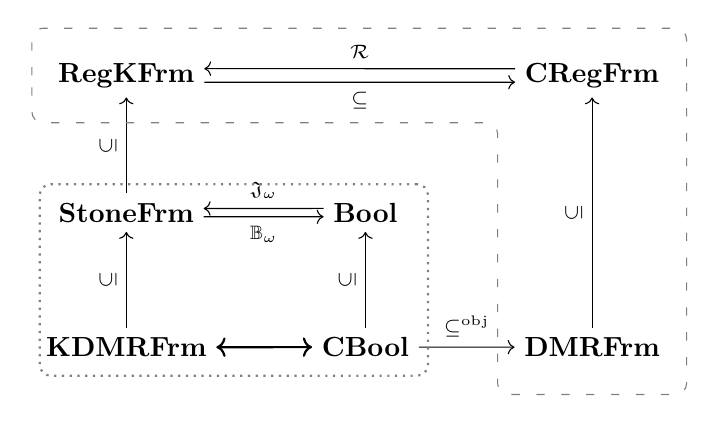
\begin{tikzpicture}[descr/.style={fill=white,inner sep=2.5pt}]
    \tikzset{
      mymx/.style={
        matrix of nodes,
        % nodes=block,
        row sep=3.5em,
        column sep=3.5em,
      },
      lbl/.style={
        % above,
        below,
        auto,
        % pos=0.15,
        % sloped, % make the text follow the path
        %execute at begin node={$}, % begin math mode, for the minus signs etc.
        %execute at end node={$}, % end math mode
      }
    }
    \tikzstyle{bigbox} = [draw=gray, thick, rounded corners, rectangle]

    \pgfmathsetmacro{\H}{1.2}
    \pgfmathsetmacro{\W}{0.6}

    \matrix (m) [mymx]
        { \RegKFrm & & \CRegFrm \\
          \StoneFrm & \Bool & \\
          \categoryStyle{KDMRFrm} & \categoryStyle{CBool} & \categoryStyle{DMRFrm} \\
        };
    \path[->,font=\scriptsize,every node/.style=lbl]
        (m-2-1)     edge node {\InclUp} (m-1-1)
        (m-3-1)     edge node {\InclUp} (m-2-1)
        (m-3-3)     edge node {\InclUp} (m-1-3)
        (m-3-2)     edge node {\InclUp} (m-2-2)
        (m-3-2)     edge node {$ \subseteq^{\text{obj}}$} (m-3-3)

        % Stone duality
        (m-2-2) edge[transform canvas={yshift=1.5pt}]  node[swap] {\JO}  (m-2-1)
        (m-2-1) edge[transform canvas={yshift=-1.5pt}] node[swap] {\BcO} (m-2-2)

        % Compact. Reflection
        (m-1-1.355) edge node[swap] {$\subseteq$} (m-1-3.185)
        (m-1-3.175) edge node[swap] {\C} (m-1-1.5);

    \path[<->, thick]
        (m-3-1) edge node {} (m-3-2);


    \node[bigbox, dotted] [fit = (m-2-1) (m-3-2)] {};
    \draw[gray, rounded corners, loosely dashed]
           ($(m-1-1) + (-\H,   0)$)
        -- ($(m-1-1) + (-\H, +\W)$)
        -- ($(m-1-3) + (+\H, +\W)$)
        -- ($(m-3-3) + (+\H, -\W)$)
        -- ($(m-3-3) + (-\H, -\W)$)
        -- ($(m-1-3) + (-\H, -\W)$)
        -- ($(m-1-1) + (-\H, -\W)$)
        -- ($(m-1-1) + (-\H,   0)$);
\end{tikzpicture}
\end{center}

Where the symbol $\subseteq^{\text{obj}}$ denotes inclusion of objects of one category to another. New categories in the diagram: \categoryStyle{CBool} denotes the category of complete Boolean algebras and \emph{all} Boolean homomorphisms. The category \categoryStyle{KDMRFrm} is the category of all extremally disconnected Stone spaces, or in other words all compact De Morgan regular frames, and \emph{all} frame homomorphisms. \categoryStyle{RegKFrm} denotes the category of compact regular frames, \categoryStyle{CRegFrm} the category of completely regular frames.

In the diagram, Stone duality is drawn in the area surrounded by the dotted rectangle and the compactification is drawn in the area surrounded by the dashed curve. As we know from the discussion above, the construction on objects is exactly the same for both marked parts of the diagram. However, the Stone correspondence is an isomorphism of categories, whereas the compactification is just a coreflection (of completely regular frames onto compact regular frames).

Taking the frame of all regular ideals of a bounded pseudocomplemented lattice is a general construction of compact frames. A natural question arises: Is it possible to extend the category \ComplBool{} to a wider subcategory of \categoryStyle{DMRFrm} and again obtain an isomorphism of categories witnessed by \R{}? From the following diagram we can see why it is not possible.

\begin{diagram}
    \categoryStyle{KDMRFrm} \ar[<->, thick]{r}{} & \categoryStyle{CBool} \ar{r}{\subseteq^{\text{obj}}} & \categoryStyle{DMRFrm} \ar[bend right=20,swap]{ll}{\restr{\C}{\categoryStyle{DMRFrm}}} \\
    \ExtrStoneFrm \ar[yshift=-0.2em,swap]{r}{\BcI}\ar{u}{\InclUp} & \ComplBool \ar[yshift=0.2em,swap]{l}{\JI} \ar{u}{\InclUp} \ar{ru}{\subseteq}
\end{diagram}

Objects of \categoryStyle{CBool} are in correspondence with objects of \categoryStyle{KDMRFrm}. On the other hand, \R{} provides a coreflection of the category \categoryStyle{DMRFrm} onto \categoryStyle{KDMRFrm}. Since \ComplBool{} is a subcategory of \categoryStyle{CBool}, we cannot hope to expand the correspondence by extending the category \ComplBool{} into a wider subcategory of \categoryStyle{DMRFrm}.

% we have in the category all (regular) De Morgan frames as objects, we cannot expect from \R{} to form an isomorphism, because we know, the category of compact (regular) De Morgan frames is (non--isomorphically) coreflexive in the category of (regular) De Morgan frames~\ref{p:extrDiscPreserv} (certainly, there exists a non--compact (regular) De Morgan frame).

% TODO Compare compactification in classical and in point-free setting. Mention that \JI{} correspond to compactification, the topology of Ult is isomorphic to ideal lattice of Boolean algebra and that this was known~\cite{monk1989handbook}.
% (note: Taken from the big picture of Stone duality)

\section{Booleanization}

\begin{definition}\label{d:Booleanization}
    Let $H$ be a Heyting algebra, by \DEF{Booleanization} of $H$ we mean the set
    $$
    \DEFSYM{Booleanization}{\Bo H} = \Set{ a^{**} | a \in H }.
    $$
\end{definition}

\begin{proposition}
    Let $H$ be a Heyting meet--semilattice, then $\Bo H$, with joins and meets defined
    $$ a \sqcup b = (a^* \wedge b^*)^* \quad\text{and}\quad a\sqcap b = a \wedge b,$$

    \noindent is a Boolean algebra.
\end{proposition}
\begin{proof}
    First, we will show that the operations $\sqcap$ and $\sqcup$ really are the meet and join for $\Bo H$. Let $a,b,c \in \Bo H$:

    \begin{itemize}
        \item From~\ref{p:pseudcomplProperties}, $a\sqcap b = a^{**}\wedge b^{**} = (a\wedge b)^{**} \in \Bo H$.
        \item Whenever $a,b \leq c$, then $a^*, b^*\geq c^*$ and so $a^*\wedge b^*\geq c^*$, hence $a\sqcup b = (a^*\wedge b^*)^* \leq c^{**} = c$. And trivially, $a\sqcup b \in \Bo H$.
    \end{itemize}

    For $a \in \Bo H$: $a^* = a^{***} \in \Bo H$ too, $a\sqcup a^* = (a^*\wedge a^{**})^* = 0^* = 1$ and also $a\sqcap a^* = a\wedge a^* = 0$. Hence, each element is complemented and $\Bo H$ is a Boolean algebra.
\end{proof}

\num\label{p:propertiesBooleanization}
    Let $L$ be a frame, the mapping defined as $a \mapsto a^{**}$ is a nucleus:
    \begin{enumerate}[label=(N\arabic*)]
        \item $a \leq a^{**}$: it is a standard inequality (Lemma~\ref{p:pseudcomplProperties});
        \item $(a \leq b \implies a^{**} \leq b^{**})$: holds, since taking pseudocomplements is antitone;
        \item $a^{**\;**} = a^{**}$: simply from $a^* = a^{***}$; and
        \item $(a \wedge b)^{**} = a^{**} \wedge b^{**}$: it is again a standard equality.
    \end{enumerate}

    Therefore, by~\ref{p:nuclProp}, $\Bo L$ is a sublocale of $L$ and consequently a complete Boolean algebra. As a drirect consequence of~\ref{p:nuclProp}, the mapping
    $$\text{\DEFSYM{BetaL}{$\beta_L$}}\colon L \to \Bo L,\quad a \mapsto a^{**},$$

    is a frame homomorphism.

\begin{block}{Note}
    $\Bo L$ is the smallest dense sublocale of $L$; and joins are also given by the following formula $(a \vee b)^{**}$ (since $a \mapsto a^{**}$ is a nucleus).
\end{block}


\begin{definition}\label{d:BooleanizationMorph}
    For a frame homomorphism $f\colon H \to K$, set \DEFSYM{BooleanizationMorph}{$\Bo f$}$\colon \Bo H \to \Bo K$ to be the mapping
    $$\Bo f\colon a \mapsto f(a)^{**}.$$
\end{definition}

\num\label{p:boolenizationCond} The following Proposition is taken from~\cite{banaschewski1996booleanization}.
\begin{proposition*}
    Let $f\colon L \to M$ be a frame homomorphism, then $\Bo f$ is a frame homomorphism such that the following diagram commutes
    \begin{diagram}
        L \ar{r}{\beta_L} \ar{d}{f} & \Bo L \ar{d}{\Bo f}\\
        M \ar{r}{\beta_M}           & \Bo M
    \end{diagram}
    if and only if $f(a^{**}) \leq f(a)^{**}$ for all $a \in L$.
\end{proposition*}
\begin{proof}
    First observe that
    \begin{align}
        f(a^{**})^{**} = f(a)^{**} \iff f(a^{**}) \leq f(a)^{**},\quad\text{for all } a\in L.\label{e:2202iff20leq02}\tag{W.O.}
    \end{align}

    $\Leftarrow$ is straightforward and the $\Rightarrow$ implication follows simply from $f(a^{**}) \leq f(a^{**})^{**} $. Commutativity of the diagram above is precisely the equality $f(a^{**})^{**} = f(a)^{**}$.

    The last thing we need to show is that $f(a^{**}) \leq f(a)^{**}$ implies that $\Bo f$ is a frame homomorphism. It is straightforward to see that $\Bo f$ preserves $0$, $1$ and $\sqcap$. For $\sqcup$--preserving, take $a, b \in \Bo L$ and infer
    $$(\Bo f)(a)\sqcup (\Bo f)(b) = (f(a)^{**}\vee f(b)^{**})^{**} \geq f(a^{**}\vee b^{**})^{**} = f(a\vee b)^{**} = (\Bo f)(a\sqcup b),$$

    \noindent where the middle and the last equality hold by~(\oldref{e:2202iff20leq02}). The opposite inequality follows from: $f(a)^{**}\vee f(b)^{**}\leq f(a\vee b)^{**}$, thus $\Bo f$ is a Boolean homomorphism.

    We will show that $\Bo f$ preserves arbitrary joins. Again using~(\oldref{e:2202iff20leq02}), we get
    $$ (\Bo f)(\bigsqcup A) = f((\bigvee A)^{**})^{**} = f(\bigvee A)^{**} = (\bigvee f[A])^{**}. $$

    Now, take any $a\in A$, from $f(a) \leq \bigvee f[A]$ we have $f(a)^{**} \leq (\bigvee f[A])^{**}$. Since $a$ was chosen arbitrary, we also have $\bigvee_{a\in A} f(a)^{**} \leq (\bigvee f[A])^{**}$ and therefore $(\bigvee_{a\in A} f(a)^{**})^{**} \leq (\bigvee f[A])^{**}$. The opposite inequality is trivial, hence $\bigsqcup (\Bo f)[A] = (\bigvee f[A])^{**}$.

    To sum up everything, we have
    $$ \bigsqcup (\Bo f)[A] = (\bigvee f[A])^{**} = (\Bo f)(\bigsqcup A),$$
    \noindent which is what we wanted.
\end{proof}

\begin{proposition}\label{p:BooleanizationFunctor}
    Let $\p C$ be a subcategory of the category of frames and frame homomorphisms satisfying (\oldref{e:2202iff20leq02}). Then

    $$\Bo\colon \p C \to \ComplBool,$$

    \noindent defined on objects as is in~\ref{d:Booleanization} and on morphisms as is in~\ref{d:BooleanizationMorph}, is a functor.
    % TODO do not reference inside a proof -- ref{e:2202iff20leq02}
\end{proposition}
\begin{proof}
    From~\ref{p:propertiesBooleanization} we know $\Bo L$ is a complete Boolean algebra. As a direct implication of Proposition~\ref{p:boolenizationCond} we get that for any morphism $f\colon L \to M$ in $\p C$, the following diagram commutes.

    \begin{diagram}
        L \ar{r}{\beta_L} \ar{d}{f} & \Bo L \ar{d}{\Bo f}\\
        M \ar{r}{\beta_M}           & \Bo M
    \end{diagram}

    \noindent $\Bo f$ is a frame homomorphisms, but it is also a complete Boolean homomorphisms, as we know from~\ref{p:kappaCompleteBAfromMeets}. Since the following diagram also commutes, for any morphisms $f, g$, we can see $\Bo$ respect morphisms composition.

    \begin{diagram}
        L \ar{r}{\beta_L}
          \ar{d}{f}
          \ar[bend right]{dd}[swap]{gf} &
        \Bo L \ar{d}[swap]{\Bo f}
              \ar[bend left]{dd}{\Bo (gf)}\\

        M \ar{r}{\beta_M} \ar{d}{g} & \Bo M \ar{d}[swap]{\Bo g}\\
        N \ar{r}{\beta_N}           & \Bo N
    \end{diagram}

    Finally, for any identity frame homomorphism $i_L$, $\Bo i_L$ is the identity on $\Bo L$. Consequently, $\Bo$ is a functor.
\end{proof}

\begin{lemma}\label{p:basicalMorphs}
    Let $f\colon L \to M$ be a frame homomorphism and $a \in L$ such that $a^{**}\vee a^* = 1$, then
    $$ f(a^{**})^* = f(a^*).$$

    In particular, for $a = a^{**}$ we have
    $$ f(a)^* = f(a^*).$$
\end{lemma}
\begin{proof}
    From the assumptions we see the following holds
    \begin{align*}
        f(a^{**}) \vee f(a^*) &= f(a^{**} \vee a^*) = 1, \\
        f(a^{**}) \wedge f(a^*) &= f(a^{**} \wedge a^*)  =  0.
    \end{align*}

    Hence $f(a^{**})$ is complemented and $f(a^*)$ is its complement. From distributivity of $M$ we know, complements are unique, hence $f(a^*) = f(a^{**})^*$.
\end{proof}

\num\label{p:BooleanizationFunctorOnExtrDSF} For any frame homomorphism between two extremally disconnected Stone frames $f\colon L\to M$, by Lemma~\ref{p:basicalMorphs}, $f(a^{**})^* = f(a^*)$ for all $a\in L$. Observe, we have
    \begin{align*}
        f(a^{**})^* = f(a^*)\text{ and }f(a^{**}) \leq f(a)^{**} \iff f(a^*) = f(a)^*,\quad\text{for all } a\in L.\label{e:1001}\tag{N.O.}
    \end{align*}

    \noindent (Indeed, the $f(a^*) \leq f(a)^*$ is always true and $f(a^*) = f(a^{**})^* \geq f(a)^{***} = f(a)^*$, the opposite direction is straightforward).

    Hence, for a category of extremally disconnected frames, in order to satisfy conditions of Proposition~\ref{p:BooleanizationFunctor}, we need to restrict morphisms only to those frame homomorphisms satisfying~(\oldref{e:1001}).

    However, this is exactly the case with morphisms of the category \ExtrStoneFrm{}. For a frame homomorphism, to be basically complete is precisely the same as to satisfy~(\oldref{e:1001}).

\begin{conclusion*}
    $\Bo\colon \ExtrStoneFrm \to \ComplBool$ is a functor.
\end{conclusion*}

In literature are frame homomorphisms satisfying (\oldref{e:2202iff20leq02}) called \DEF{weakly open} and frame homomorphisms satisfying (\oldref{e:1001}) are called \DEF{nearly open}~\cite{banaschewski1994variants}.
% TODO topological interpretation

\begin{observation}\label{p:boEQbc}
    $\Bo L = \BcI L$ for any extremally disconnected Stone frame $L$.
\end{observation}
\begin{proof}
    $\Bo L \supseteq \BcI L$ holds always. Let $x \in \Bo L$, then $x = x^{**}$ and from extremal disconnectedness also $x^{**}\vee x^*=1$, hence $x \in \BcI L$.
\end{proof}


Until the end of this section, we will use Lemma~\ref{p:idealsFrame} frequently without further referencing.

\begin{proposition}
    The functor $\Bo\circ\JI$ is naturally equivalent to the identity functor on \ComplBool{}.
\end{proposition}
\begin{proof}
    Let $B$ be a Boolean frame. We see $J \in \Bo\JI(B)$ iff $J = J^{**} = \downset \bigvee J$.

    Denote by \DEFSYM{istar2}{$\tilde i_B$}$\colon B \to \Bo\JI(B)$ the mapping $a \mapsto \downset a$. From the previous Observation we know the definitions of $\tilde i_B$ and $i_B$ coincide, therefore by~\ref{p:BoolEquivalence} $\tilde i_B$ is a Boolean isomorphism. From~\ref{p:completePartUnits}, $\tilde i_B$ is a morphisms of \ComplBool{}.

    Now, for any complete Boolean algebras $A$ and $B$, for any complete Boolean homomorphism $f\colon A \to B$, the following diagram commutes
    \begin{diagram}
        A \ar{r}{\tilde i_A} \ar{d}[swap]{f} & \Bo\JI(A) \ar{d}{\Bo\J(f)}\\
        B \ar{r}{\tilde i_B}                 & \Bo\JI(B)
    \end{diagram}

    \noindent Indeed, we have
    $$
    \Bo\JI(f)(\downset a) = (\downset f[\downset a])^{**} = \downset f(a)^{**} = \downset f(a).
    $$

    Hence, the collection $\tilde i_*$ of complete Boolean homomorphisms forms a natural equivalence between $\Bo\JI$ and the identity functor on \ComplBool.
\end{proof}

\begin{proposition}\label{p:JOBoIdentity}
    The functor $\JI\circ\Bo$ is naturally equivalent to the identity functor on \ExtrStoneFrm{}.
\end{proposition}
\begin{proof}
    Let $L$ be an extremally disconnected Stone frame. Similarly to the general case, define \DEFSYM{vstar2}{$\tilde v_L$}$\colon \JI\Bo(L) \to L$ as
    $$ \tilde v_L\colon I \mapsto \bigvee I.$$

    \noindent From Observation~\ref{p:boEQbc}, we know the definitions of $\tilde v_L$ and $v_L$ are the same, and $\tilde v_L$ is a frame isomorphism by~\ref{p:StoneFrmEquivalence}. From~\ref{p:completePartUnits}, $\tilde v_L$ is a morphism of \ExtrStoneFrm.

    Further, let $L$ and $M$ be extremally disconnected Stone frames and let $f\colon L \to M$ be a basically complete frame homomorphism. The following diagram commutes
    \begin{diagram}
        \JI\Bo(L) \ar{d}[swap]{\JI\Bo(f)} \ar{r}{\tilde v_L} & L \ar{d}{f} \\
        \JI\Bo(M) \ar{r}{\tilde v_M}    & M
    \end{diagram}

    To show that, let $I \in \JI\Bo(L)$. First observe, for $x\in I$, $x = x^{**}$ and since $L$ is extremally disconnected, $x\vee x^* = 1$. Therefore, $f(x^*) = f(x)^*$ by Lemma~\ref{p:basicalMorphs}. Now, we can compute
    $$
    (\JI\Bo)(f)(I) = \downset \Set{ f(x)^{**} | x \in I } = \downset \Set{ f(x) | x \in I} = \downset f[I].
    $$

    \noindent And from that, we see
    $$
    \tilde v_M((\JI\Bo)(f)(I)) = \bigvee \downset f[I] = \bigvee f[I] = f(\bigvee I) = f(\tilde v_L(I)).
    $$

    The conclusion follows from commutativity of the diagram above.
    The collection $\tilde v_*$ of basically complete frame homomorphisms is a natural equivalence between $\JI\Bo$ and the identity functor on \ExtrStoneFrm.
\end{proof}


\num From \ref{p:BooleanizationFunctorOnExtrDSF}---\ref{p:JOBoIdentity}, we obtain the main result of this section.

\begin{theorem*}
    The functors \Bo{} and \JI{} provide an isomorphism between the categories \\\ExtrStoneFrm{} and \ComplBool{}.
\end{theorem*}

% TODO
% \num Observe that $\Bo$ provides an isomorphism precisely for this part of Stone correspond. For a frame $L$, $\Bo L$ is always a complete Boolean algebra and the frame $\JI\Bo(L)$ is extremally disconnected.

% TODO and by \ref{e:1001} we cannot hope to ommit condition to have weakly open frame homomorphismsa?


% \chapter{More about DeMorgan Frames}
% \section{Uniformity and metrizability}
% \section{Non--metrizability of compactification}
% \begin{lemma}
%     For $L$ normal frame: $\sigma(x)\vee\sigma(x) = \sigma(x\vee y)$.
% \end{lemma}

\chapter{Conclusion}
TODO or Further work?


\nocite{*}
\bibliographystyle{plain}
\bibliography{refs.bib}

\clearpage
% \addcontentsline{toc}{chapter}{Index}
\printindex
\end{document}
